%--------------------------------------------------------------
% tesi.tex 
%--------------------------------------------------------------
% Corso di Laurea in Informatica 
% http://if.dsi.unifi.it/
% @Facolt\`a di Scienze Matematiche, Fisiche e Naturali
% @Universit\`a degli Studi di Firenze
%--------------------------------------------------------------
% - template for the main file of Informatica@Unifi Thesis 
% - based on Classic Thesis Style Copyright (C) 2008 
%   Andr\'e Miede http://www.miede.de   
%--------------------------------------------------------------

\documentclass[twoside,openright,titlepage,fleqn,
,	headinclude,12pt,a4paper,BCOR5mm,footinclude,table]{scrbook}
%--------------------------------------------------------------
\newcommand{\myItalianTitle}{Titolo In Italiano\xspace}
\newcommand{\myEnglishTitle}{Title In English\xspace}
% use the right myDegree option
\newcommand{\myDegree}{Corso di Laurea Magistrale in Informatica\xspace}
%\newcommand{\myDegree}{
	%Corso di Laurea Specialistica in Scienze e Tecnologie 
    %dell'Informazione\xspace}
\newcommand{\myCurriculum}{Data Science\xspace}
\newcommand{\myName}{Federico Schipani\xspace}
\newcommand{\myProf}{Marco Bertini\xspace}
\newcommand{\myOtherProf}{Nome Cognome\xspace}
\newcommand{\mySupervisor}{Nome Cognome\xspace}
\newcommand{\myFaculty}{
	Scuola di Scienze Matematiche, Fisiche e Naturali\xspace}
\newcommand{\myUni}{\protect{
	Universit\`a degli Studi di Firenze}\xspace}
\newcommand{\myLocation}{Firenze\xspace}
\newcommand{\myTime}{Anno Accademico 2018-2019 (spero)\xspace}
\newcommand{\myVersion}{Version 0.1\xspace}
%--------------------------------------------------------------
\PassOptionsToPackage{dvipsnames}{xcolor}
\PassOptionsToPackage{pdftex}{graphicx}
\usepackage[italian]{babel}
\usepackage[utf8]{inputenc} 
\usepackage[T1]{fontenc} 
\usepackage[square,numbers]{natbib} 
\usepackage[fleqn]{amsmath}  
\usepackage{ellipsis}
\usepackage{listings}
\usepackage{subfig}
\usepackage{caption}
\usepackage{appendix}
\usepackage{siunitx}
\usepackage{url}
\usepackage{epigraph}
\usepackage{amsthm}
%--------------------------------------------------------------
\usepackage{dia-classicthesis-ldpkg}
%--------------------------------------------------------------


%
% Options for classicthesis.sty:
% tocaligned eulerchapternumbers drafting linedheaders 
% listsseparated subfig nochapters beramono eulermath parts 
% minionpro pdfspacing
\usepackage[eulerchapternumbers,linedheaders,subfig,beramono,eulermath,
parts]{classicthesis}
%--------------------------------------------------------------
\newlength{\abcd} % for ab..z string length calculation
% how all the floats will be aligned
\newcommand{\myfloatalign}{\centering} 
\setlength{\extrarowheight}{3pt} % increase table row height
\captionsetup{format=hang,font=small}
%--------------------------------------------------------------
% Layout setting
%--------------------------------------------------------------
\usepackage{geometry}
\geometry{
	a4paper,
	ignoremp,
	bindingoffset = 1cm, 
	textwidth     = 13.5cm,
	textheight    = 21.5cm,
	lmargin       = 3.5cm, % left margin
	tmargin       = 4cm    % top margin 
}


\usepackage{tikz}
\usetikzlibrary{arrows}
\usetikzlibrary{positioning}
\usetikzlibrary{decorations.markings}
\usetikzlibrary{fit}
\usetikzlibrary{calc}
\tikzset{main node/.style={circle,fill=blue!20,draw,minimum size=1cm,inner sep=0pt},
            }

\tikzstyle{vecArrow} = [thick, decoration={markings,mark=at position
1 with {\arrow[semithick]{open triangle 60}}},
double distance=1.4pt, shorten >= 5.5pt,
preaction = {decorate},
postaction = {draw,line width=1.4pt, white,shorten >= 4.5pt}]
\theoremstyle{definition}
\newtheorem{definition}{Definizione}[section]
%--------------------------------------------------------------
\begin{document}
\definecolor{c338dd8}{RGB}{51,141,216}
\definecolor{cdf672a}{RGB}{223,103,42}
\definecolor{cc1433c}{RGB}{193,67,60}
\frenchspacing
\raggedbottom
\pagenumbering{roman}
\pagestyle{plain}
%--------------------------------------------------------------
% Frontmatter
%--------------------------------------------------------------


%--------------------------------------------------------------
% titlepage.tex (use thesis.tex as main file)
%--------------------------------------------------------------
\begin{titlepage}
	\begin{center}
   	\large
      \hfill
      \vfill
      \begingroup
         \includegraphics[scale=0.15]{logo/LOGO}\\
%			\spacedallcaps{\myUni} \\ 
			\myFaculty \\
			\myDegree \\ 
			\vspace{0.5cm}
         \vspace{0.5cm}    
           
      \endgroup 
      \vfill 
      \begingroup
      	\color{Maroon}\spacedallcaps{\myItalianTitle} \\ $\ $\\
      	\spacedallcaps{\myEnglishTitle} \\ 	
	\bigskip
      \endgroup
      \spacedlowsmallcaps{\myName} \\ $\ $\\
      \spacedlowsmallcaps{\myProf}
      \vfill 
      \vfill
    
      \vfill
      \vfill
      \myTime
      \vfill                      
	\end{center}        
\end{titlepage}   
%--------------------------------------------------------------
% back titlepage
%--------------------------------------------------------------
   \newpage
	\thispagestyle{empty}
	\hfill
	\vfill
	\noindent\myName: 
	\textit{\myItalianTitle,} 
	\myDegree, \textcopyright\ \myTime
%--------------------------------------------------------------
% back titlepage end
%--------------------------------------------------------------

\pagestyle{scrheadings}
%--------------------------------------------------------------
% Mainmatter
%--------------------------------------------------------------
\pagenumbering{arabic}
% use \cleardoublepage here to avoid problems with pdfbookmark
%\include{intro} % use \myChapter command instead of \chapter
%\cleardoublepage\myPart{Part I}
%\include{chapter01}
%\cleardoublepage\myPart{Part II}
%\include{chapter02}
%\include{chapter03}
\tableofcontents
\listoftables
\listoffigures
\addcontentsline{toc}{chapter}{Introduzione}
\chapter*{Introduzione}
Il \textit{Machine Learning}, detto anche Apprendimento Automatico, nasce come diramazione dell'intelligenza artificiale e trova  campi di applicazione sempre più ampi nel mondo contemporaneo.  
In passato questa disciplina era limitata dall'hardware disponibile ma ora, grazie all'avvento di \ac{gpu} sempre più potenti o addirittura hardware dedicato, riusciamo ad usare modelli sempre più complessi e precisi in diversi ambiti della vita quotidiana. 

Il trend attuale prevede l'utilizzo sempre maggiore di Reti Neurali artificiali. Una Rete Neurale è un modello matematico che per molti versi cerca di ricalcare la funzionalità 
di un cervello umano allo scopo di sostituirlo per quei compiti che possono essere definiti \textit{ripetitivi}. 

Il cervello umano è composto da neuroni connessi tra di loro che formano una rete, uno di questi componenti è schematizzato sinteticamente in Figura \ref{fig:neurone}. 
\begin{figure}[]
    \centering
    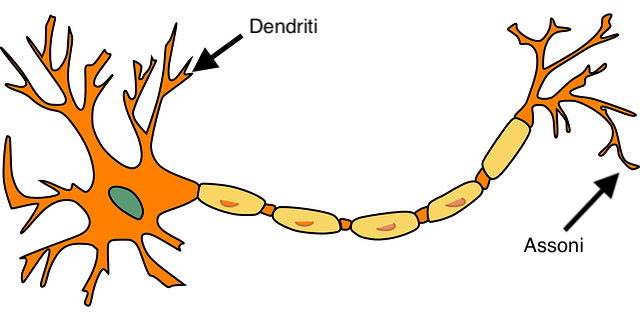
\includegraphics[width = 0.7\textwidth]{images/neurone.png}
    \caption{Schema di un neurone}
    \label{fig:neurone}
\end{figure}
All'interno di un neurone gli impulsi elettrici scorrono fino ad arrivare dall'assone, dopodiché sono modulati dalle sinapsi ed infine arrivano ai dendriti degli altri neuroni connessi ad esso formando una rete.

Una rete neurale artificiale, similmente ad un cervello umano, quindi è composta da tanti neuroni artificiali analoghi ad un neurone biologico; essi ricevono in input dei dati che vengono 
modulati da dei \textit{pesi} ed infine passando per una \textit{funzione di attivazione} vengono restituiti in output ad altri neuroni artificiali. Lo schema di un neurone artificiale è in Figura \ref{fig:neuron_artificial}; gli input $x_i$ vengono combinati linearmente tramite i corrispettivi pesi $w_i$ ed infine passando per la funzione di attivazione $\sigma$ restituiscono un output. 
\begin{figure}
    \centering
    \begin{tikzpicture}
        \node[rectangle](x1){$x_1$};
        \node[rectangle, below of = x1](x2){$x_2$};
        \node[rectangle, below of = x2](x3){$x_3$};
        \node[rectangle, below of = x3](x4){$x_4$};
        \node[rectangle, below of = x4](x5){$x_5$};
        \node[circle, draw, ultra thick, fill=gray!20, right = 2.5cm of x3](sigma) {$\Sigma$};
        \draw [->] (x1) edge[] node[ fill=white, anchor=center, pos=0.35] {$\omega_1$} (sigma);
        \draw [->] (x2) edge[] node[ fill=white, anchor=center, pos=0.35] {$\omega_2$} (sigma);
        \draw [->] (x3) edge[] node[ fill=white, anchor=center, pos=0.35] {$\omega_3$} (sigma);
        \draw [->] (x4) edge[] node[ fill=white, anchor=center, pos=0.35] {$\omega_4$} (sigma);
        \draw [->] (x5) edge[] node[ fill=white, anchor=center, pos=0.35] {$\omega_5$} (sigma);
        \node[circle, draw, ultra thick, fill=gray!20, right = 4cm of sigma](sigmam) {$\sigma$};
        \draw [->, thick] (sigma)  edge[] node[ fill=white, anchor=center, pos=0.5] {$y = \omega^T x$} (sigmam);
        \node[right = 1cm of sigmam](out) {$\sigma(y)$};
        \draw[->, thick] (sigmam) -- (out);
    \end{tikzpicture}
    \caption{Neurone artificiale}
    \label{fig:neuron_artificial}
\end{figure}

Un esempio di utilizzo delle reti neurali può essere la guida autonoma: molte case costruttrici, integrando hardware molto potente in situazioni critiche, riescono ad  adottare reti neurali per realizzare veicoli sempre più sicuri e per ridurre l'intervento umano in casi di emergenza o durante lunghi viaggi. 
Lo stato dell'arte in ambito consumer sulla guida autonoma è stato raggiunto dall'americana \textit{Tesla} con il suo \textit{AutoPilot} che, 
grazie a nove telecamere posizionate attorno alla vettura, riesce a raggiungere un livello di autonomia mai visto prima.
Altri utilizzi possono essere la videosorveglianza, dove riconoscere intrusioni di persone o vetture all'interno di un perimetro diventa un compito critico e molto importante che fino a pochi anni fa era prerogativa esclusiva di esseri umani. 
Le reti neurali sono usate anche per controllo qualità, \textit{speech recognition}, \textit{sentiment analysis} e per vari altri compiti. 


Il nostro interesse sarà focalizzato sul miglioramento del riconoscimento di oggetti su immagini rilevate nello spettro termico in quanto offrono un vantaggio in condizioni di scarsa visibilità rispetto alle immagini tradizionali; l'elaborato è dunque strutturato come segue:
\begin{itemize}
    \item nel Capitolo 1 presenta un introduzione all'argomento riguardante la rilevazione di oggetti, fornendo quindi una panoramica delle metodologie, tecniche e modelli più importanti e di come si sono evolute nel corso del tempo. 
    \item all'interno Capitolo 2 si descrive l'organizzazione del sistema su cui abbiamo lavorato per lo sviluppo della tesi, in particolare si affrontano più analiticamente i dataset e le tecniche utilizzate. 
    \item il Capitolo 3 riguarda invece gli esperimenti effettuati usando come base ciò che è stato descritto nel precedente capitolo. 
\end{itemize}


\chapter{Object Detection}
L'Object Detection è un \textit{task} legato al mondo della \textit{computer vision}
che consiste nel rilevare e classificare istanze di oggetti in immagini o video.

Negli ultimi anni, grazie soprattutto all'avvento delle \ac{gpu}, c'è stato un 
incremento notevole del potere computazionale. Questo ha portato a sviluppare tecniche 
sempre più raffinate allo scopo di raggiungere prestazioni sempre migliori. 

Lo sviluppo di hardware sempre più potente ha portato l'interesse verso modelli di  \textit{Deep Learning}. 
In questo capitolo cercheremo di contestualizzare, anche storicamente, tecniche, modelli ed evoluzioni
nel campo della \textit{Object Detection}. 
La letteratura sui detector è molto disomogenea e variegata, prenderemo quindi come 
riferimento i lavori di Licheng Jiao \textit{et al.} 
\cite{DBLP:journals/corr/abs-1907-09408} e 
Zhengxia Zou \textit{et al.} \cite{DBLP:journals/corr/abs-1905-05055}.


\section{Storia della object detection}
\label{sec:history_obj}
Una prima, ma importante distinzione va fatta tra il periodo pre e post \textit{deep learning}. Il primo periodo va dagli inizi degli anni $2000$ fino al $2014$. Il secondo periodo, dove hanno preso il sopravvento tecniche basate sul \textit{deep learning}, va dal $2014$ fino ai nostri giorni. Quest'ultime tecniche possono essere a loro volta divise in altre due categorie, \textit{One Stage Detector} e \textit{Two Stage Detector} (sarà il caso di tradurre in italiano?) il cui sviluppo procede in maniera parallela. In Figura \ref{fig:history_object_detection} è presente uno schema riassuntivo con tutte le pietre miliari raggiunte durante lo sviluppo di tecniche per il rilevamento di oggetti.
\begin{figure}
    \centering
    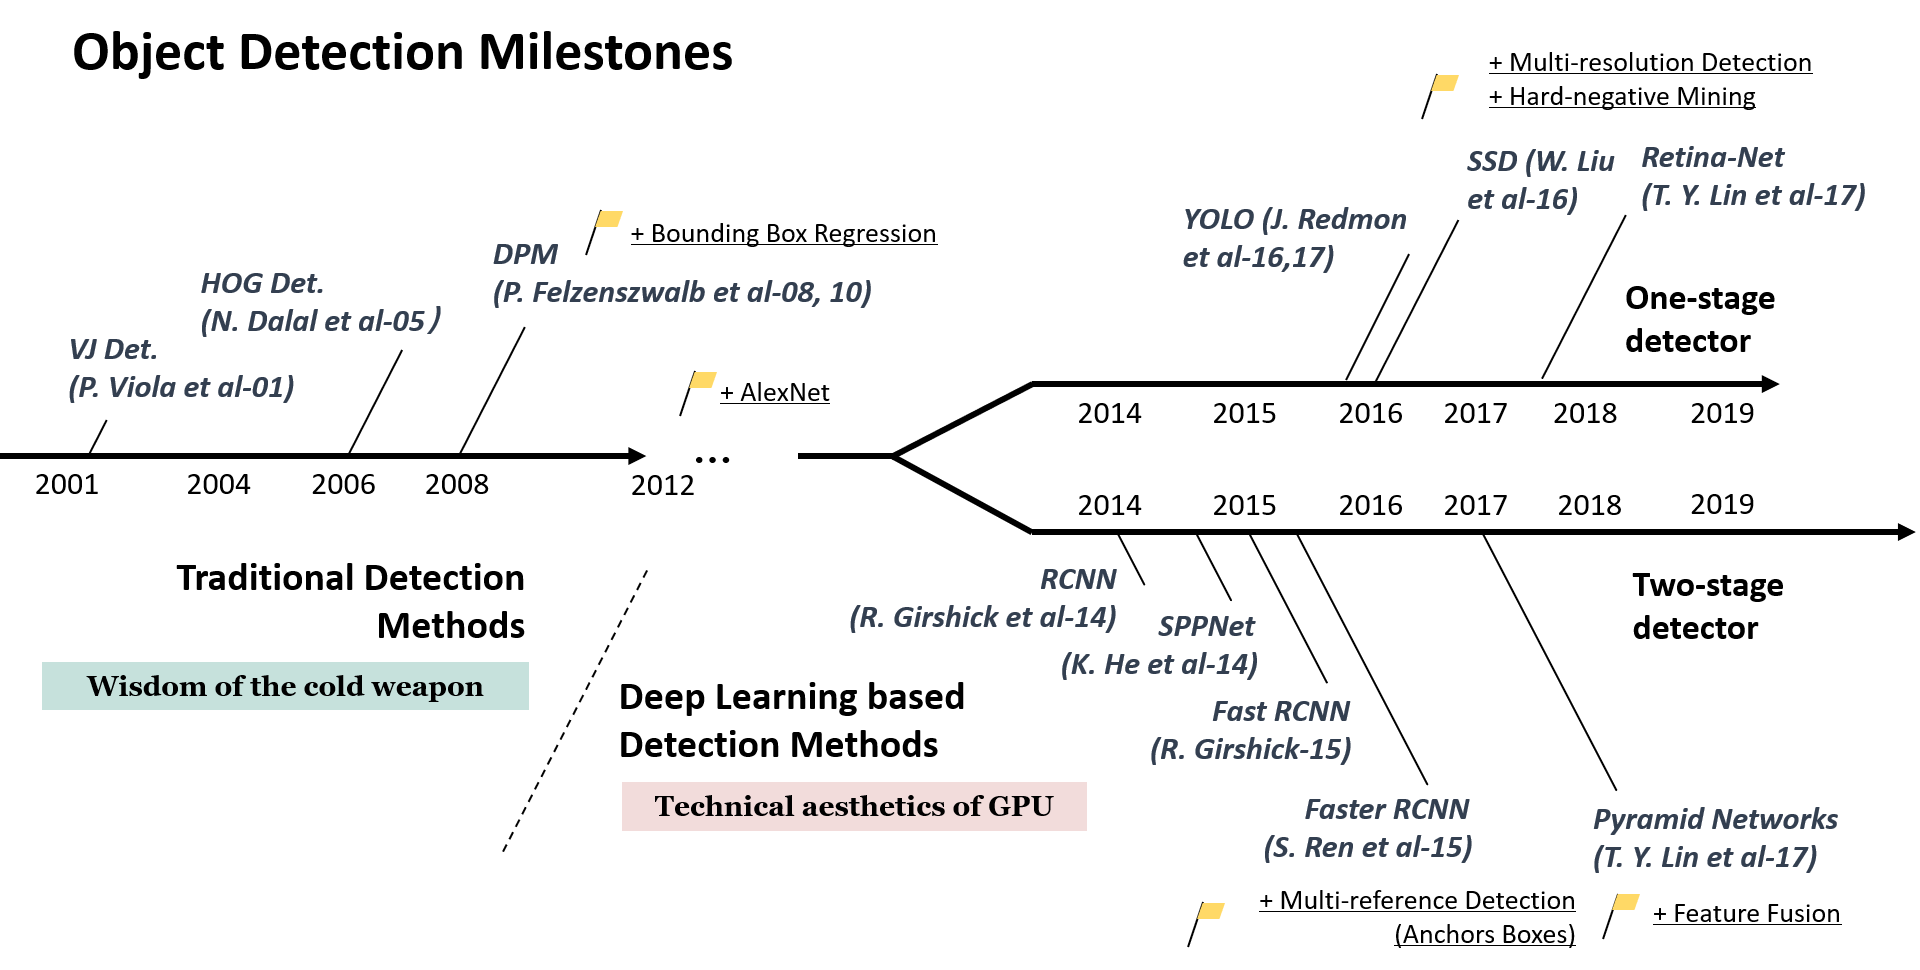
\includegraphics[width=\textwidth]{images/mile-stones.png}
    \caption{Storia della Object Detection \cite{DBLP:journals/corr/abs-1905-05055}}
    \label{fig:history_object_detection}
\end{figure}
\subsection{Evoluzione delle tecniche}
Durante questo ventennio i detector più famosi sono stati costruiti usando come mattoncini delle tecniche sviluppate ed affinate via via nel tempo. Queste tecniche sono di diverso tipo ed hanno subito evoluzioni di cui faremo una disamina nel proseguio di questa sottosezione.
\subsubsection{Prime tecniche}
Storicamente una delle prime tecniche si basava sul una teoria cognitiva chiamata \textit{Recognition by Components} \cite{biederman1987recognition}, ed è stata per molto tempo la base di alcuni lavori riguardanti il riconoscimento di immagini e la rilevazione di oggetti \cite{felzenszwalb2008discriminatively, fischler1973representation, leibe2008robust}.   

Nel passato alcuni ricercatori hanno formulato soluzioni al problema usando misure di similarità tra le componenti di un oggetto, tra la forma o i contorni, tra cui \textit{Distance Transforms} \cite{gavrila1999real}, \textit{Shape Contexts} \cite{belongie2002shape} e \textit{Edgelet} \cite{wu2005detection}.

I risultati iniziali erano molto promettenti, tuttavia quando la rilevazione è diventata più complicata queste tecniche hanno iniziato a mostrare i propri limiti, motivo per cui il passaggio al Machine Learning è stato quasi naturale. Le prime metodologie basate su questo approccio risalgono ad un periodo inquadrabile prima del $1998$, in questo caso la detection si basava su modelli statistici costruiti sopra le caratteristiche visibili che accomunano gli oggetti da rilevare. 
Il primo di questi modelli statistici, nato nel $1991$ e chiamato \textit{Eigenfaces} \cite{turk1991eigenfaces, pentland1994view}, riesce in laboratorio a riconoscere volti in tempo reale.

Successivamente, fino al $2005$, l'evoluzione ha portato a tecniche in cui si cambiava radicalmente la rappresentazione dell'immagine, detta anche insieme delle feature. Inizialmente lo scopo era apprendere come trasformare un immagine da insieme di pixel a insieme di coefficenti \textit{wavelet}. Grazie alla sua efficienza, tra tutte le trasformate, quella a prendere piede fu la \textit{Haar wavelet}. Dal $2005$ al $2012$ c'è stato un passaggio a rappresentazioni basate sul gradiente. 

Intorno al $1990$ iniziano a fare capolino le prime \ac{CNN} \cite{vaillant1994original} le quali però non hanno avuto grandi applicazioni per via dell'elevato costo computazionale rispetto alle risorse disponibili ai tempi. I modelli realizzati con \ac{CNN} non potevano essere quindi molto profondi, e per questo avevano forti limitazioni. Un lavoro che ai tempi tentava di ridurre il l'elevato costo computazionale è \textit{space displacement network} \cite{lecun1998gradient}. L'idea era di estrarre una rappresentazione dell'immagine in un solo passaggio ed è stata realizzata estendendo i layer della \ac{CNN}. Storicamente le \ac{CNN} di cui si parla nel lavoro di LeCun \textit{et al.} possono essere considerate un po' le antenate di quelle che attualmente chiamiamo \ac{FCN} \cite{long2015fully} \cite{chen2014semantic}
\subsubsection{Detection multiscala}
\label{subsec:multiscale_detection}
Uno degli aspetti più interessanti della ricerca si basa sulla rilevazione di oggetti con diverse misure o diverse proporzioni. Come è possibile vedere in Figura \ref{fig:multi_scale_history} la soluzione a questo problema ha attraversato varie fasi.
\begin{figure}
    \centering
    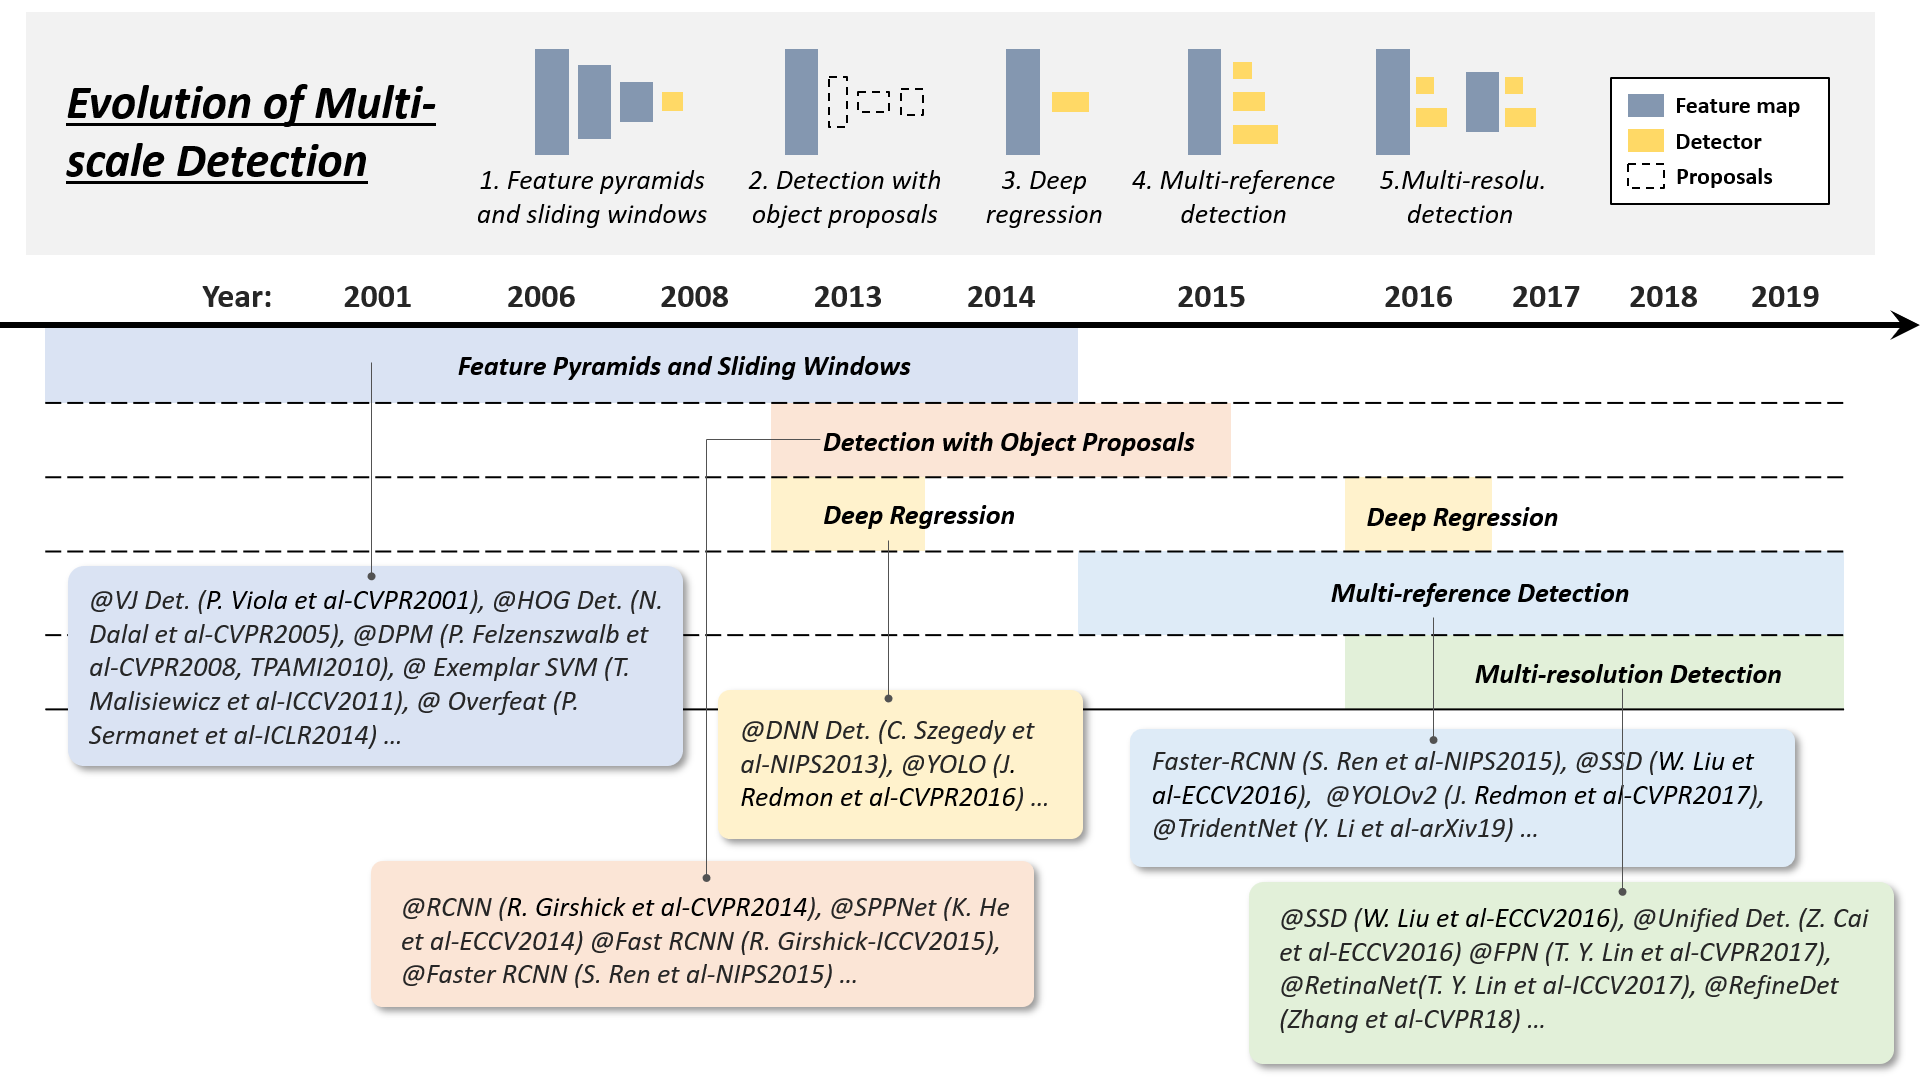
\includegraphics[width=\textwidth]{images/evol-multiscale.png}
    \caption{Evoluzione della detection multiscala \cite{DBLP:journals/corr/abs-1905-05055}}
    \label{fig:multi_scale_history}
\end{figure}
\paragraph{Feature piramidali e finestre scorrevoli}
L'idea dietro questa tecnica è abbastanza basilare, infatti dopo aver estratto le feature da un'immagine quello che viene fatto è far scorrere una finestra rettangolare di dimensione generalmente fissa per effettuare il rilevamento e la classificazione di oggetti. 

Dal $2004$ al $2014$ sono stati creati un sacco di detector basati su questa filosofia, il problema è che erano stati disegnati con l'intento specifico di rilevare oggetti con proporzioni fisse. Ricercatori come R. Girshick \textit{et al.} iniziarono a cercare soluzioni a questo problema, arrivando a formulare un modello mistura \cite{felzenszwalb2009object} composto da più modelli addestrati su oggetti con differenti proporzioni. Sono state sviluppate anche altre soluzioni, basate questa volta sull'addestrare modelli separati per ogni istanza di oggetto dell'insieme di addestramento \cite{malisiewicz2011ensemble, malisiewicz2011exemplar}. Le limitazioni di tutte queste tecniche risiedono nel fatto che i dataset più moderni sono molto diversificati, quindi nel corso del tempo sono diventate sempre meno precise ed utilizzabili. Ciò ha portato allo sviluppo di \textit{Object Proposal}.
\paragraph{Object Proposal}
Il primo avvistamento di \textit{Object Proposal} risale al $2010$ in un task di rilevazione di oggetti \cite{alexe2010object}.
Possiamo definire una regione come un'area di un immagine contenente pixel che hanno caratteristiche comuni tra di loro. L'idea dietro questa tecnica è creare regioni non etichettate con classi che potenzialmente possono contenere qualunque tipo di oggetto, e lo scopo è riuscire a rilevare oggetti di varie misure e scale pur non dovendo necessariamente svolgere una ricerca esaustiva con finestre scorrevoli.

Per ottenere queste regioni di pixel su un immagine ci sono vari modi, discussi in parte da J. Hosang \textit{et al.} in \cite{hosang2015makes}.
\paragraph{Deep Regression}
Questa tecnica, sviluppata dal $2013$ al $2016$ si basa sull'idea di predirre direttamente le coordinate della \ac{BB} contenente l'oggetto usando come feature quelle estratte da un modello di \textit{deep learning} \cite{redmon2016you}. Il vantaggio fondamentale di questo approccio è l'efficienza e la velocità di implementazione, mentre uno svantaggio è la bassa accuratezza di localizzazione specialmente su piccoli oggetti.
\paragraph{Multi Reference Detection}
Questo approccio è il più usato per il rilevamento di oggetti con scale differenti e si basa sull'uso di un insieme di finestre rettangolari, che possono variare in dimensione e proporzioni, applicate sull'immagine, dette anche \textit{Anchor Boxes} \cite{ren2015faster, liu2016ssd, redmon2017yolo9000}. Sulla base di queste regioni rettangolari viene poi effettuata una predizione della \ac{BB}. 
\paragraph{Multi Resolution Detection}
Negli ultimi anni un altro approccio che ha preso piede si basa sul rilevare oggetti con dimensioni differenti a layer differenti, sfruttando quindi la struttura di un modello a strati \cite{liu2016ssd, lin2017feature, zhang2018single, cai2016unified}. Basti pensare alle \ac{CNN} che nel corso della propagazione dell'immagine in input, grazie alla loro composizione, formano una rappresentazione piramidale dell'input. Diventa quindi più facile rilevare oggetti grandi nei layer più profondi e viceversa diventa più facile rilevare oggetti piccoli nei layer meno profondi. 
\subsubsection{Regressione basata su Bounding Box}
Questo insieme di metodologie ha lo scopo di affinare la posizione delle \ac{BB} basandosi sulle rilevazioni effettuate tramite \textit{Object Proposal} o \textit{Anchor Boxes}, descritte precedentemente. Uno schema riassuntivo dell'evoluzione tecnica di questi approcci è in Figura \ref{fig:bbox_history}.
\begin{figure}
    \centering
    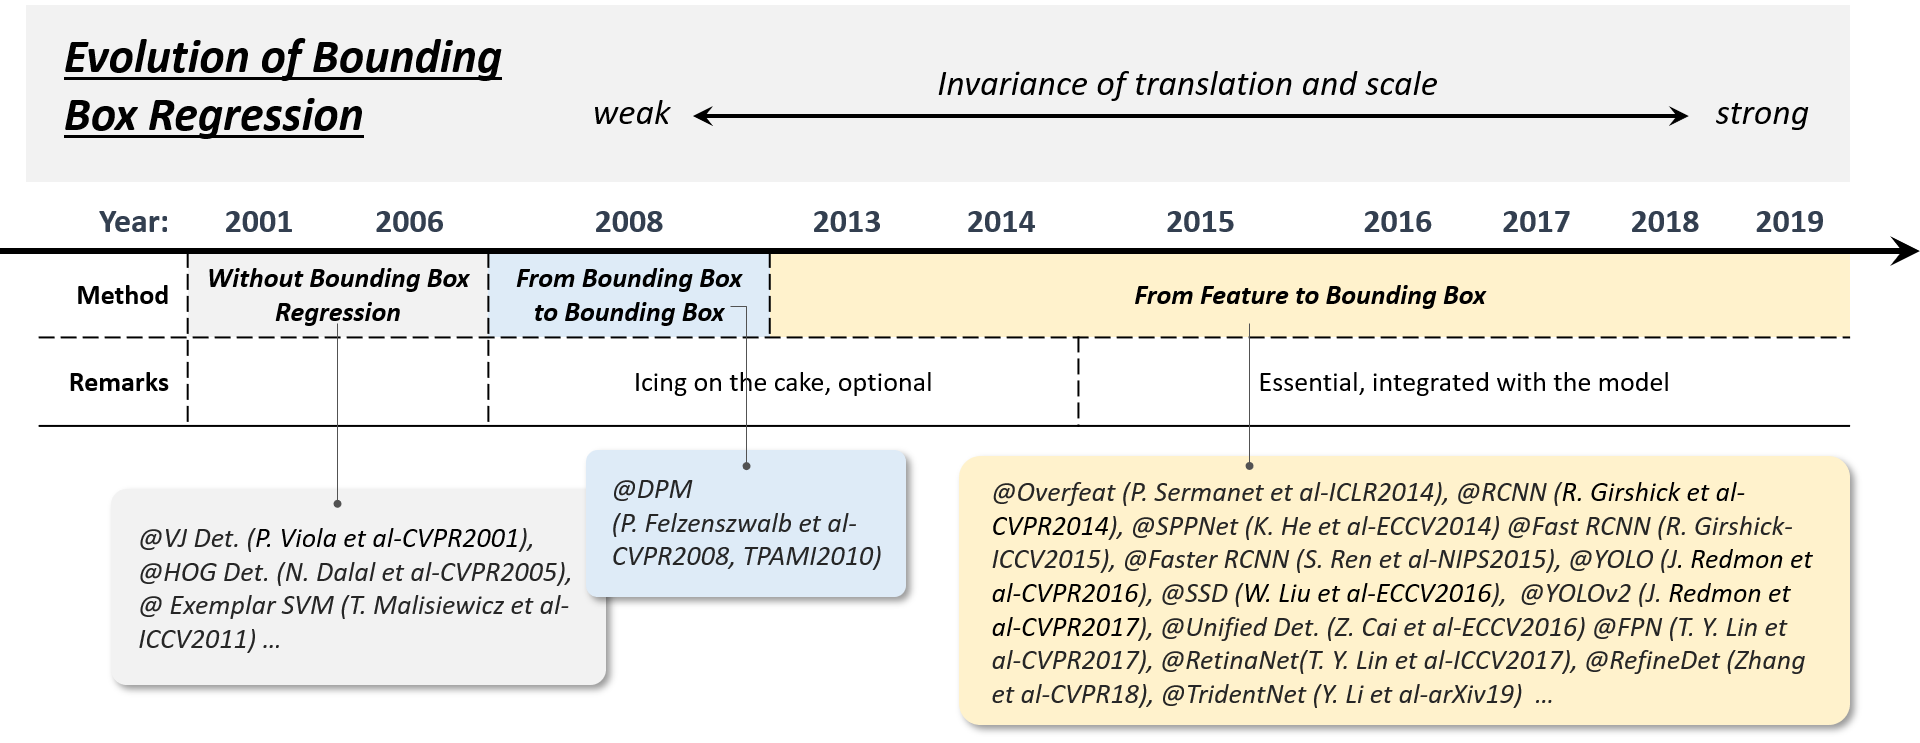
\includegraphics[width=\textwidth]{images/evol-bbreg.png}
    \caption{Evoluzione della regressione basata su \ac{BB} \cite{DBLP:journals/corr/abs-1905-05055}}
    \label{fig:bbox_history}
\end{figure}

I primi detector non raffinavano in alcun modo la posizione delle \ac{BB}, anzi molte volte usavano direttamente l'output derivato da un algoritmo basato su finestre scorrevoli. L'unico modo per ottenere rilevazioni più precise era quindi costruire modelli piramidali molto densi e assicurarsi di far scorrere la finestra lungo tutta l'immagine.
\paragraph{Da Bounding Box a Bounding Box}
I primi ad usare una forma di regressione per aumentare la precisione sulle \ac{BB} sono stati P. F. Felzenszwalb \textit{et al.} in DPM \cite{5255236} formulando la soluzione con il metodo dei minimi quadrati. Per scendere più nel dettaglio dobbiamo considerare un modello con feature piramidali.
In breve nel modello proposto in \cite{5255236} l'implementazione è effettuata tramite una funzione $g(z)$ che associa ad un vettore di feature le coordinate $(x_1, y_1)$ e $(x_2, y_2)$ della \ac{BB}. Dopo la fase di addestramento del modello viene usato l'output di $g(z)$ per un'ulteriore fase di addestramento nella quale tramite il metodo dei minimi quadrati si impara ad effettuare predizioni più corrette su $x_1, y_1, x_2 \text{ e } y_2$ partendo da $g(z)$. Bisogna però specificare che questo tipo di ottimizzazione è stata implementato a livello di post-processing, quindi risulta del tutto opzionale.
\paragraph{Da feature a Bounding Box}
A differenza del tipo di ottimizzazione proposto in precedenza, con l'introduzione delle \textit{Faster RCNN} \cite{ren2015faster} nel $2015$ la regressione è implementata allo stesso livello nel quale viene effettuata anche la rilevazione stessa dell'oggetto. L'addestramento quindi non è più una fase separata ed opzionale, bensì diventa parte fondamentale e procede in parallelo con l'addestramento del modello.  Inoltre, sempre confrontandolo con quanto detto prima, vengono usate anche diverse funzioni di loss da minimizzare che risultano più robuste rispetto a quella usata nei minimi quadrati. Degli esempi possono essere la \textit{smooth-L1} o la \textit{root-square}.

\subsubsection{Valutazione del contesto}
Generalmente gli oggetti che vengono rilevati dai sistemi di detection sono immersi in un contesto. Il cervello umano durante la fase cognitiva trae vantaggio dal riconoscere un contesto, motivo per cui le tecniche spiegate nel proseguio di questa sottosezione provano a emulare questa capacità degli umani. Una breve storia di come queste tecniche si sono evolute è in Figura \ref{fig:context_history}.
\begin{figure}
    \centering
    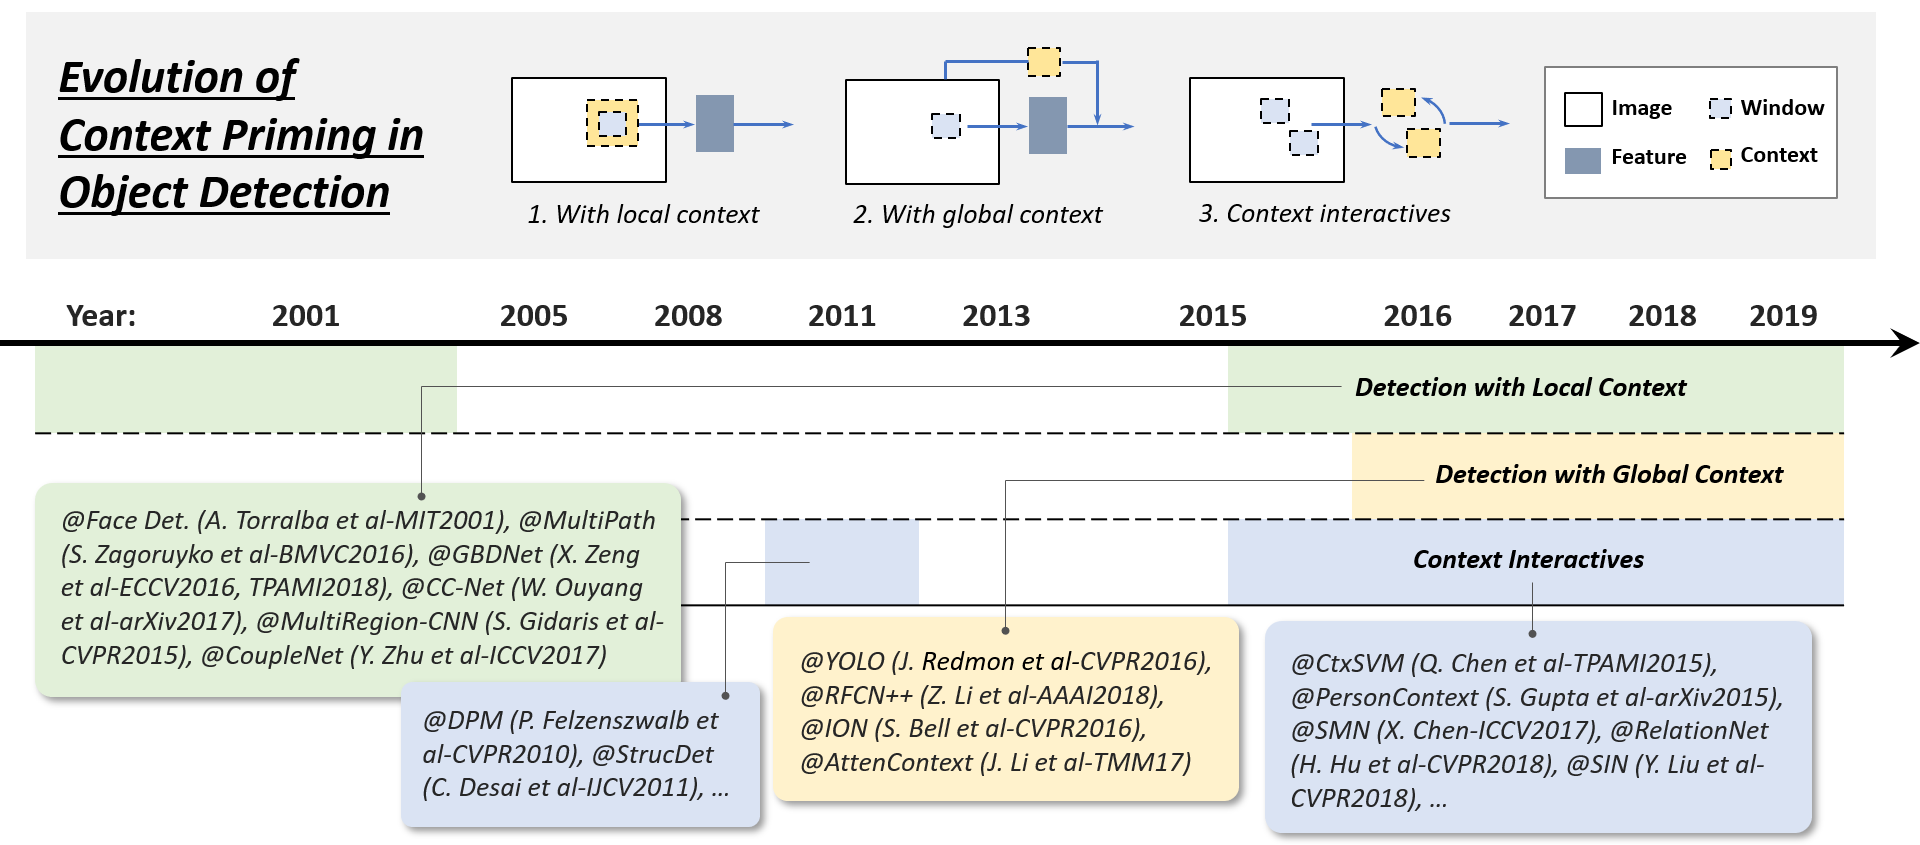
\includegraphics[width=\textwidth]{images/evol-context.png}
    \caption{Evoluzione del context priming \cite{DBLP:journals/corr/abs-1905-05055}}
    \label{fig:context_history}
\end{figure}
\paragraph{Contesto locale}
Per contesto locale si intendono tutte le informazioni visive che fanno parte dell'area più prossima ai contorni di un oggetto. Sin dagli anni 2000 Sinha e Torralba in \cite{torralba2001detecting} hanno provato che includere del contesto locale migliora le prestazioni ai fini del rilevamento di volti. Dalal e Triggs in \cite{dalal2005histograms} hanno dimostrato che introdurre una piccola porzione di sfondo migliora i risultati anche nel rilevamento dei pedoni. 
\paragraph{Contesto globale}
Il contesto globale può essere considerato come una fonte di informazione aggiuntiva riguardante la scena in cui l'oggetto da rilevare è immerso. Un metodo usato all'inizio per inglobare nella detection informazioni sul contesto globale era realizzare delle statistiche che riassumevano la totalità degli elementi compresi nella scena \cite{divvala2009empirical}. In lavori più moderni catalogabili come modelli di \textit{deep learning} sono state intraprese due strade, la prima è quella di inglobare il contesto tramite campi recettivi sempre più ampi, a volte anche più dell'immagine stessa \cite{redmon2016you} o  usare l'operazione di \textit{pooling} delle \ac{CNN} \cite{li2018r}. La seconda via per ottenere informazioni dal contesto globale è pensare ad esso come un flusso di informazioni sequenziali ed usare \ac{RNN} \cite{bell2016inside, li2016attentive}. 
\paragraph{Contesto derivato dalle interazioni}
L'ultima contestualizzazione che si può dare ad un oggetto riguarda le sue interazioni con ciò che lo circonda. Per interazioni si possono intendere tutte quei vincoli o dipendenze che può avere l'obbiettivo della rilevazione. Recentemente in alcuni lavori sono state analizzate questo tipo di informazioni contestuali ai fini del miglioramento della detection. Questi miglioramenti possono essere divisi in due macrocategorie, la prima di queste è quella in cui si esplorano le relazioni tra oggetti individuali \cite{felzenszwalb2009object, desai2011discriminative, song2011contextualizing, chen2017spatial, hu2018relation}. Nella seconda categoria fanno parte i lavori nei quali vengono prese in considerazione le relazioni che ci sono tra gli oggetti e la scena che li circonda \cite{gupta2015exploring, liu2018structure}.
\subsubsection{Non Maximum Suppression}
Per \ac{NMS} si fa riferimento a tutte quelle tecniche di post processing per ridurre il fenomeno delle \ac{BB} duplicate. Questo fenomeno si concretizza quando, per la stessa rilevazione, ci sono più \ac{BB} che circondano l'oggetto con confidenze molto simili tra di loro. L'evoluzione di queste tecniche nel corso del tempo è possibile vederla in Figura \ref{fig:NMS_history}. 
\begin{figure}
    \centering
    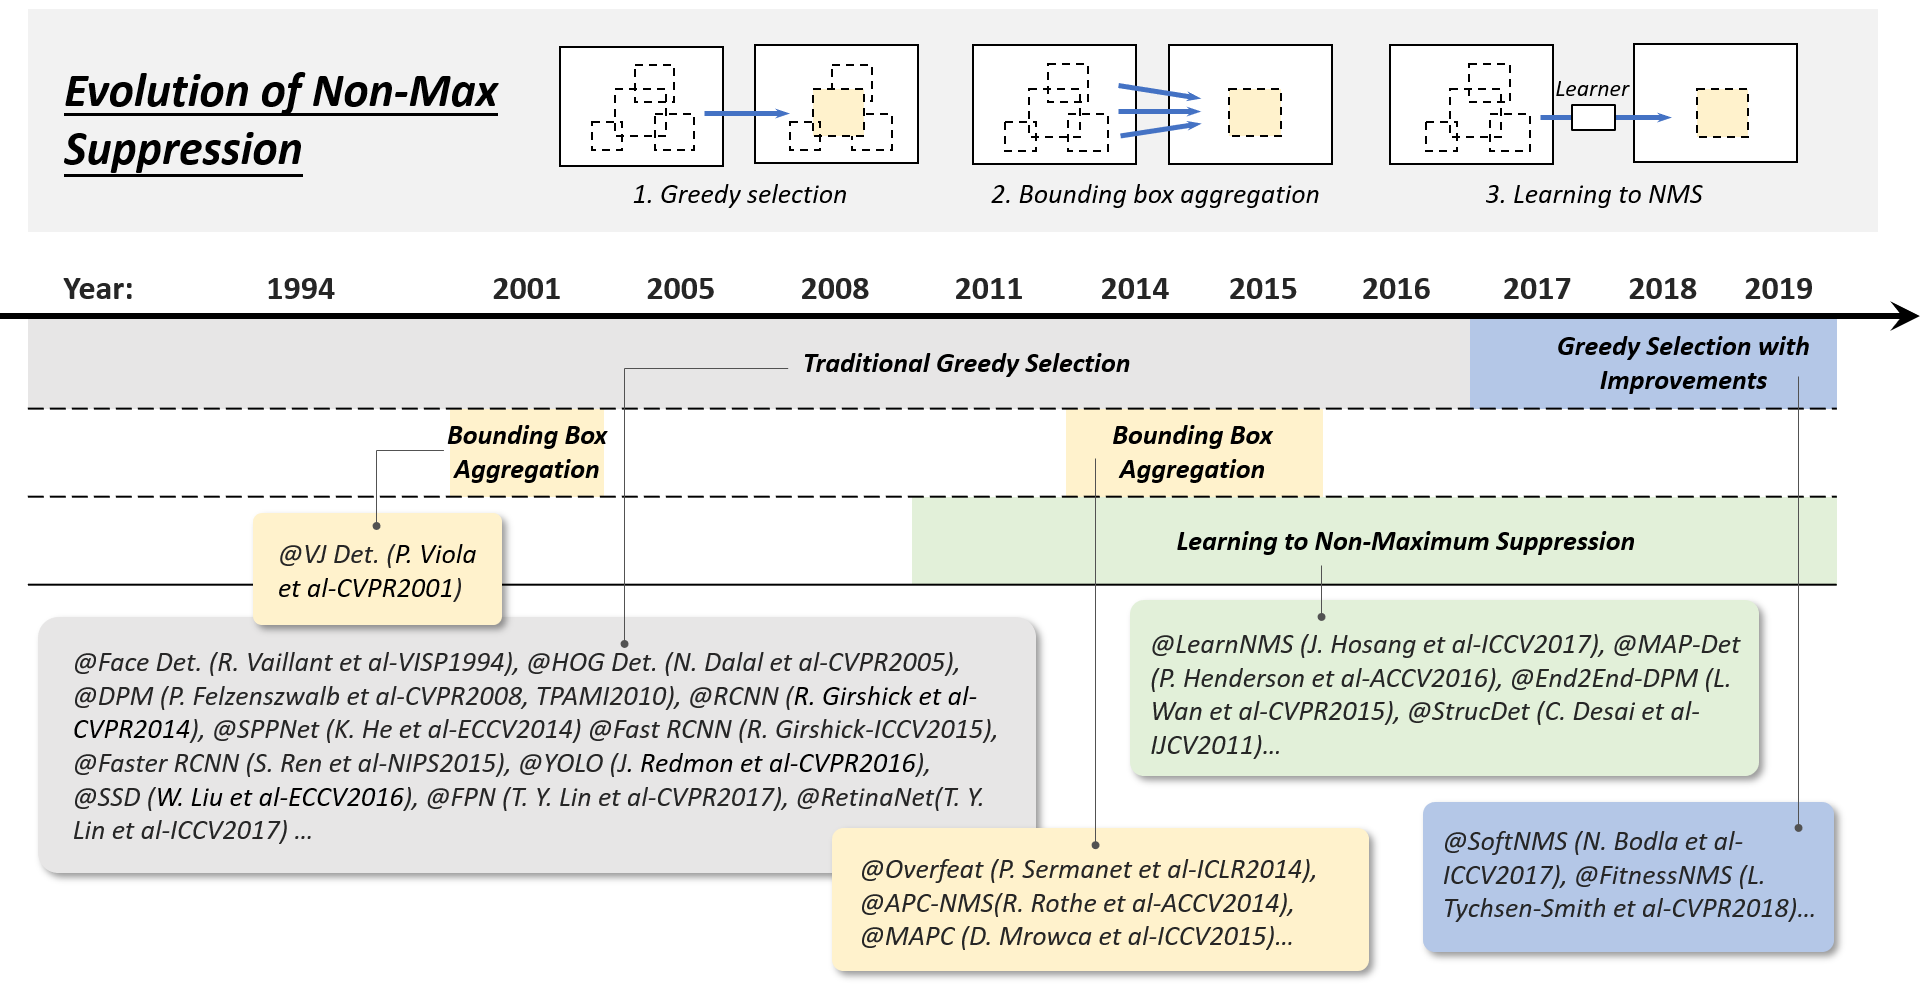
\includegraphics[width=\textwidth]{images/evol-nms.png}
    \caption{Evoluzione della Non Maximum Suppression \cite{DBLP:journals/corr/abs-1905-05055}}
    \label{fig:NMS_history}
\end{figure}


\paragraph{Greedy}
La maniera più semplice per attuare la \ac{NMS} è con un algoritmo di tipo \textit{greedy}, infatti per un insieme di \ac{BB} sovrapposte si considera solamente quella con la confidenza massima, mentre le altre vengono scartate. La sua semplicità, che da un certo punto di vista può anche essere vista come un punto di forza, può anche essere fonte di debolezze in quanto un algoritmo \textit{greedy} non sempre porta all'ottimalità. Si possono infatti verificare casi in cui la \ac{BB} con massima confidenza non ricopre tutto l'oggetto, o ancora peggio le \ac{BB} di oggetti vicini tra di loro possono essere scartate erroneamente.


\paragraph{Aggregazione di Bounding Box}
L'aggregazione di \ac{BB} vicine tra di loro è un altro approccio per attuare la \ac{NMS} \cite{viola2001rapid, sermanet2013overfeat, rothe2014non, mrowca2015spatial}. L'aggregazione può essere fatta sia attraverso algoritmi di \textit{clustering}, sia combinando le \ac{BB} sovrapposte in un unica singola detection. 


\paragraph{Imparare ad applicare Non-maximum Suppression}
Approcci più recenti per migliorare le già sopracitate tecniche di \ac{NMS} riguardano l'apprendimento automatico \cite{wan2015end, desai2011discriminative, hosang2017learning, henderson2016end}. L'idea dietro questi metodi è trattare la \ac{NMS} alla stessa stregua di un filtro che assegna nuovi valori di confidenza a tutte le detection e quindi bisognoso anch'esso di una fase di addestramento. 

\subsubsection{Hard Negative Mining}
Uno dei problemi a cui bisogna far fronte quando si tratta la \textit{Object Detection} è lo sbilanciamento in cardinalità tra gli oggetti che vogliamo rilevare e conseguentemente classificare e tutto quello che non ci interessa. Visto che generalmente lo sfondo ricopre una buona parte dell'immagine la prima soluzione che potrebbe venire in mente per risolvere questo problema è addestrare il modello a riconoscere lo sfondo, ma questo porta a risultati pessimi durante l'addestramento in termini di efficienza. Tecniche di \ac{HNM} servono proprio a risolvere queste problematiche. Una breve storia è possibile vederla in Figura \ref{fig:HNM_history}.
\begin{figure}
    \centering
    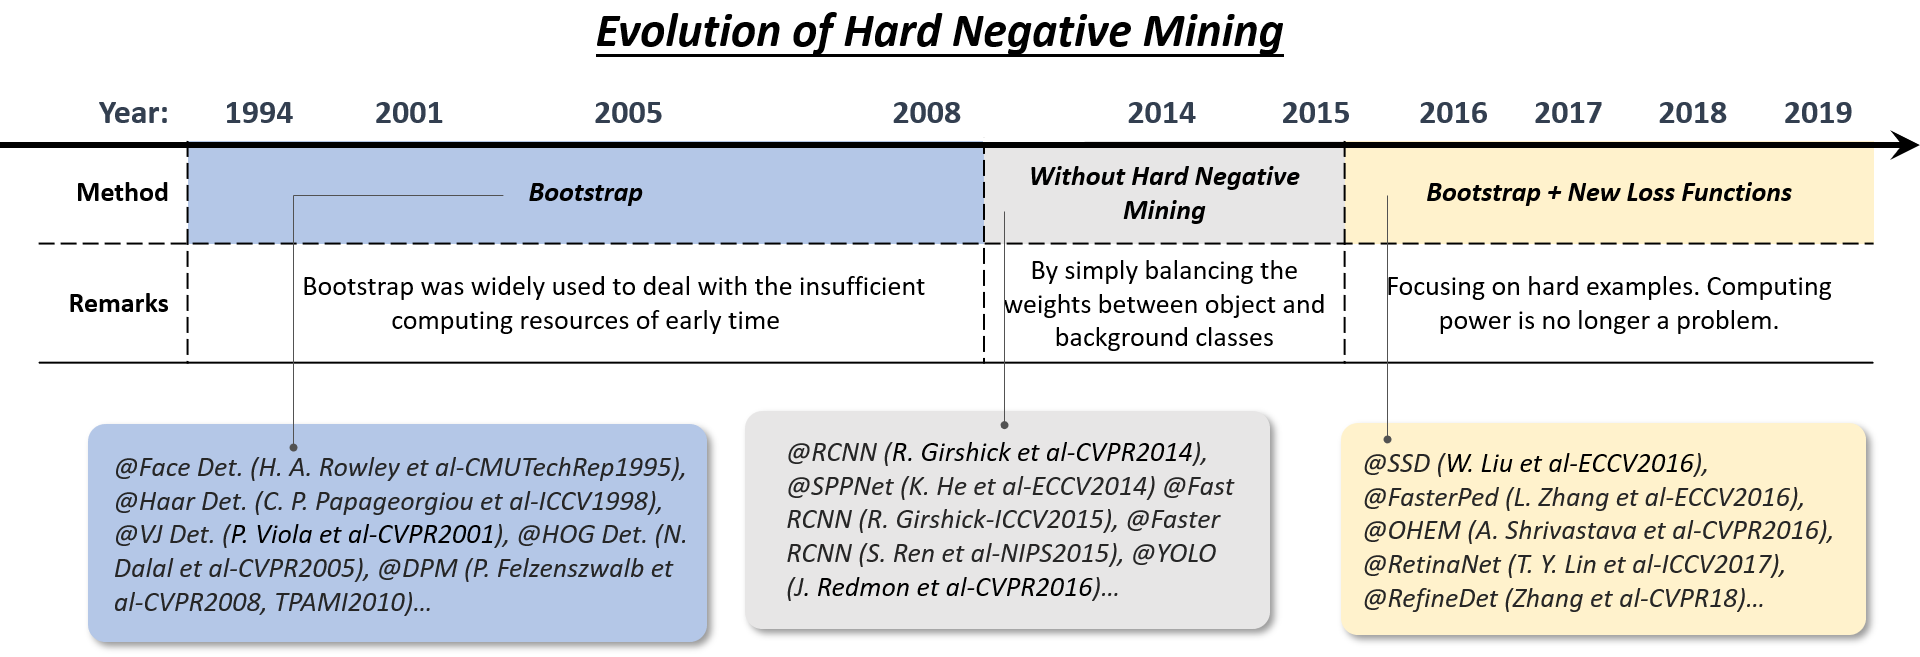
\includegraphics[width=\textwidth]{images/evol-hardnegmining.png}
    \caption{Evoluzione di Hard Negative Mining \cite{DBLP:journals/corr/abs-1905-05055}}
    \label{fig:HNM_history}
\end{figure}
\paragraph{Bootstrap}
Per Bootstrap si fa riferimento ad un gruppo di tecniche attraverso le quali si fa iniziare la fase di addestramento con piccoli esempi di sfondo. 
Successivamente quando si rilevano esempi di sfondo classificati erroneamente si aggiungono al processo di addestramento. Questo approccio risulta efficiente in quanto si evita di addestrare il modello su milioni di esempi di sfondi \cite{viola2001rapid, papageorgiou1998general, rowley1996human}.
\paragraph{HNM in detector basati su deep learning}
Recentemente modelli come Faster RCNN e \ac{YOLO} per risolvere questo problema bilanciano i pesi tra finestre con esempi negativi e positivi. Nonostante tutto però non viene risolto completamente il problema di sbilanciamento, quindi c'è stato un ritorno al \textit{bootstrap}. Un altro modo per risolvere lo sbilanciamento è l'introduzione di nuove funzioni di Loss, come ad esempio la Focal Loss in RetinaNet \cite{lin2017focal}, descritta con maggior dettaglio in Sezione \ref{subsec:focal_loss}. 




\subsection{Dataset}
L'insieme dei dati con cui addestrare e testare le performance dei modelli via via sviluppati nel corso del tempo ha subito un evoluzione. Costruire dataset sempre più grandi e con meno bias è sempre stato un obbiettivo principale che si ponevano i ricercatori, tutto ciò per realizzare dei benchmark che mettessero sempre di più a dura prova i nuovi modelli. 

Nel seguito di questa sezione analizzeremo in breve alcuni dei dataset più famosi nell'ambito della computer vision, con particolare attenzione per alcuni incentrati sulla rilevazione di pedoni. In Tabella \ref{table:dataset} è presente uno schema riassuntivo dei dataset presi in analisi.


\begin{table}[]
    \resizebox{\textwidth}{!}{%
    \begin{tabular}{|c|c|c|c|c|c|c|}
        \hline
        \textbf{Dataset}   & \textbf{Immagini} & \textbf{Totale BB} & \textbf{Classi} & \textbf{Risoluzione} & \textbf{Fonte}       & \textbf{Altre informazioni}                                                                                  \\ \hline
        Mit ped            & 500/200           & ND                 & 1               & $64 \times 128$      & ND                   & È stato il primo                                                                                             \\ \hline
        INRIA              & 1805              & ND                 & 1               & $64 \times 128$      & ND                   & \begin{tabular}[c]{@{}c@{}}Forma rudimentale di \\ Data Augmentation\end{tabular}                            \\ \hline
        Pascal VOC (2012)  & 11540/10991       & 27450 in train     & 20              & Variabile            & Web                  & Challenge                                                                                                    \\ \hline
        Caltech            & 124K/124K         & 350K totali        & 3               & $640 \times 480$     & Vettura in movimento & Ambiente cittadino                                                                                           \\ \hline
        KITTI              & 194/195           & 160K totali        & 6               & $1382 \times 512$    & Vettura in movimento & 3D, moltissime vetture                                                                                       \\ \hline
        ILSVRC             & 458K/46K          & ND                   & 200             & Variabile            & Web                  & Challenge                                                                                                    \\ \hline
        CityPersons        & 5K                & 35K                & 4               & ND                   & Altro dataset        & \begin{tabular}[c]{@{}c@{}}\ac{BB} con stesse proporzioni, \\ 50 città diverse\end{tabular} \\ \hline
        MS-COCO            & 123K/40K          & 896K in train      & 91              & Variabile            & Web                  & Ottima contestualizzazione                                                                                   \\ \hline
        OPEN IMAGES (2018) & 1,784M/125K       & 14M in train       & 600             & Variabile            & Web                  & \begin{tabular}[c]{@{}c@{}}Molte classi, molto ampio,\\  alta media di istanze per immagine\end{tabular}     \\ \hline
        EuroCity           & 28K/19K           & 250K in totale     & 9               & $1920 \times 1024$   & Vettura in movimento & \begin{tabular}[c]{@{}c@{}}Varietà nell'ambiente, \\ qualità delle immagini\end{tabular}                     \\ \hline
    \end{tabular}}
    \caption{Riassunto dei dataset analizzati, dove presente lo '/' indica la suddivisione tra train e test}
    \label{table:dataset}
\end{table}

\paragraph{MIT Ped.} Risale all'inizio del nuovo milleno ed è uno dei primi dataset che ha come scopo il riconoscimento di pedoni. Rispetto agli standard odierni risulta molto piccolo in quanto contiene circa 509 immagini usabili per l'addestramento e 200 usabili per la fase di test. \cite{papageorgiou2000trainable} 
\paragraph{INRIA} Risalente al 2005, nasce dall'esigenza di creare un dataset dove la detection diventasse più complicata rispetto a quello fatto dal MIT \cite{dalal2005histograms}. Contiene 1805 immagini ad una risoluzione di $64 \times 128$ pixel di esseri umani. 
Le immagini usate per l'insieme di training sono 2478, ovvero 1239 immagini, contenenti esempi positivi, prese dal totale più le stesse immagini ma specchiate secondo l'asse delle $y$.

\paragraph{Pascal VOC}
\ac{VOC} è collocabile in un periodo che va dal $2005$ al $2012$ \cite{everingham2010pascal, everingham2015pascal}. \ac{VOC} consiste di due parti complementari, la prima è un dataset pubblico e disponibile per esperimenti e benchmark, la seconda è una sfida annuale. Nel corso degli anni ne sono state sviluppate diverse versioni, individuabili dal pattern VOC\texttt{ANNO}. I task effettuabili su questo dataset spaziano classificazione di immagini alla object detection passando anche per il rilevamento di azioni. 

Per la sfida nel $2007$ sono state raccolte solo immagini dal social network \href{https://www.flickr.com/}{Flickr}. Le immagini sono molto variegate, ad esempio come scritto nell'articolo di presentazione del dataset \cite{everingham2010pascal} ci possono essere motociclette in diverse pose e forme, come può essere il veicolo per strada o come soggetto principale del fotogramma. 
Un altro esempio è la classe \textit{"person"}, mentre in molti dataset con questa classe ci si riferisce ad un pedone in VOC2007 con questa classe si fa riferimento ad un essere umano in diversi contesti. 

Per realizzare il dataset sono state definite delle keyword con cui effettuare query su \href{https://www.flickr.com/}{Flickr}. Queste suddette keyword sono state definite sulla base delle classi degli oggetti che si desiderava annotare. Tramite queste query sono state recuperate $500.000$ immagini, non prendendo in considerazione la data di acquisizione, il nome del fotografo, la location e via discorrendo. 
Le query venivano effettuate a gruppi di $100.000$ immagini alla volta, di cui venivano selezionate casualmente solamente fotografie che venivano effettivamente inserite nel dataset. Questa operazione è stata ripetuta fino ad ottenere la quantità desiderata di file. 
L'operazione successiva è stata quella di eliminare i duplicati o comunque immagini molto somiglianti tra di loro, una volta fatto questo sono passati ad annotarle. Di queste $500.000$ immagini agli annotatori ne sono state presentate $44.269$. Gli annotatori avevano la facoltà di scartare alcune immagini se le ritenevano non adatte ad essere annotate o avevano una confidenza bassa sull'eventuale annotazione da effettuare.

Nonostante ciò è stato scoperto un'elemento che portava a del bias all'interno del dataset. L'elemento in questione riguardava il modo in cui le immagini sono state recuperate. Quando si effettua una query su \href{https://www.flickr.com/}{Flickr} il server restituisce le immagini in ordine cronologico di upload sulla piattaforma. Il dataset è stato realizzato nel Gennaio $2007$, quindi buona parte delle immagini erano ambientate in un contesto natalizio o perlopiù invernale. Con VOC2008 il problema è stato risolto aggiungendo una data casuale all'interno della query per recuperare le immagini.  

\paragraph{Caltech Pedestrian Dataset} Il \textit{Caltech Pedestrian Dataset} \cite{dollar2009pedestrian} nasce nel 2009 ed è molto più ampio di tutti gli altri dataset visti in precedenza. Le immagini sono state ricavate da circa 10 ore di video girato a 30 frame al secondo in un ambiente urbano con traffico regolare. È quindi presente un numero di frame che è nell'ordine di grandezza di $10^6$. La telecamera con cui sono state acquisite le registrazioni è stata piazzata su un'autovettura con un guidatore che attraversava le strade di Los Angeles guidando in maniera normale. La risoluzione delle immagini è di $640 \times 480$ e come conseguenza del fatto che il sistema è stato più volte smontato e rimontato ci sono piccole variazioni nella posizione della telecamera. Il dataset è stato creato da $11$ sessioni dove in ognuna di queste venivano esplorati $5$ quartieri. Dopodiché le prime sei sessioni sono state destinate all'addestramento, mentre le rimanenti cinque sono state adibite a test set.

Sono stati annotati $250.000$ fotogrammi, per un totale di $350.000$ \ac{BB} e $2300$ pedoni univoci. Di tutti i fotogrammi, circa il $50\%$ non hanno pedoni, mentre il $30\%$ del totale ne ha almeno due. In media un pedone è visibile per un tempo di 5 secondi. Come su dataset più recenti i pedoni sono raggruppati secondo la loro distanza dal guidatore. In particolare abbiamo che i pedoni sono vicini se la loro altezza è maggiore di $80$ pixels, sono ad una distanza media se la loro altezza è compresa tra $30$ ed $80$ pixels, mentre sono consideati lontani se la loro altezza è al più $30$ pixels. Questa discretizzazione riguardante la distanza dei pedoni è stata realizzata seguendo la distribuzione delle altezze degli stessi all'interno del dataset. Sono state inoltre prese in considerazione statistiche riguardanti l'occlusione dei pedoni e la loro posizione rispetto alla telecamera.



\paragraph{KITTI}  \cite{geiger2012we} Questo dataset è realizzato a partire da hardware usato per la guida autonoma. La particolarità è che offre informazioni tridimensionali dell'ambiente grazie a dei sensori laser dedicati che mappano il territorio circostante. Per la realizzazione sono state  utilizzate due telecamere a colori con una risoluzione di $1392 \times 512$ pixels, uno scanner laser ed un localizzatore GPS con un'unità di correzione RTK, il tutto orchestrato da un calcolatore su cui girava un database in real time.  Tutto questo hardware è stato montato su una station wagon che è stata guidata per dei normali scenari cittadini. 
Inoltre le annotazioni non sono \ac{BB} in due dimensioni, ma dei parallelepipedi che avvolgono gli oggetti. Per la loro realizzazione sono stati presi annotatori umani che hanno posizionato \ac{BB} tridimensionali su oggetti come auto, furgoni, camion, tram, pedoni e ciclisti. Inoltre gli annotatori sono stati istruiti per marcare ogni \ac{BB} come visibile, semi occlusa, occlusa o troncata. 



\paragraph{ILSVRC}
Come per \ac{VOC} anche \ac{ILSVRC} \cite{russakovsky2015imagenet} è una challenge organizzata annualmente dal $2010$ al $2017$. Inoltre, sempre come per \ac{VOC} è presente un dataset pubblico disponibile per addestramenti e test. 
Come per alcuni dei dataset precedentemente introdotti le immagini state prese in parte da Flickr, con l'aggiunta però di altri motori di ricerca. In particolare andremo ad analizzare la costruzione della parte di dataset riguardante la \textit{object detection}, però il dataset contiene anche una parte dedicata alla classificazione di immagini ed un'altra parte dedicata alla rilevazione singola di oggetti all'interno dell'immagine. 

Le classi di oggetti presenti sono $200$ e sono stati scelte partendo dalle $1000$ classi usate per la classificazione di immagini. Una prima riduzione per arrivare a $494$ classi è stata inizialmente effettuata tramite l'eliminazione di label corrispondenti ad oggetti che occupavano gran parte del fotogramma o semplicemente non adatti alla \textit{object detection}. Un ulteriore operazione di unificazione tra classi simili ha portato il numero a $200$. 

Per il training set le immagini hanno tre provenienze differenti. Le prima sorgente di immagini è la parte di dataset dedicata alla rilevazione singola di oggetti. Per aggiungere ulteriori esempi negativi sono state prese ulteriori immagini da altri motori di ricerca. Le immagini provenienti da queste due prime fonti sono state annotate solamente con un sottoninsieme delle classi totali. L'ultima sorgente di immagini è la piattaforma Flickr su cui sono state fatte query generiche. 
Riguardo invece la porzione di dataset dedicata alla validazione e al test la situazione è molto simile in quanto la fonte primaria ($77\%$) è la porzione di di \ac{ILSVRC}2012 adibita alla rilevazione di oggetti singoli, a cui però sono state sottratte le immagini nel quale gli oggetti occupavano più del $50\%$ dell'area totale del fotogramma. Per aggiungere ulteriori esempi, come per il training set, sono state effettuate interrogazioni generiche su Flickr. A differenza dell'insieme di immagini di addestramento, per la validazione e il test, sono state usate tutte e $200$ le classi disponibili. 
In totale per il traning set sono presenti circa $458.000$ immagini, mentre per il validation e test set sono presenti $46.000$ fotogrammi. 
\paragraph{CityPersons} Zhang \textit{et al. } \cite{zhang2017citypersons} propongono un nuovo dataset derivante da Cityscapes \cite{cordts2016cityscapes}, ma invece che focalizzarsi sulla segmentazione delle scene in contesti urbani CityPersons è incentrato sulla rilevazione di pedoni. Infatti per ogni frame di Cityscapes sono stati annotati esseri umani tramite \ac{BB}.

Le classi usate in questo dataset sono quattro, e variano a seconda della postura del pedone. Con \texttt{pedestrian} vengono indicate le persone in piedi, che corrono o camminano, mentre con \texttt{rider} si indicano quelle persone che sono alla guida di un mezzo a due ruote. Sono presenti altre due classi per indicare le persone sedute (\texttt{sitting person}) e persone con pose inusuali (\texttt{other person}).

Viene standardizzato il processo di annotazione dei \texttt{pedestrian} e \texttt{riders} in quanto le \ac{BB} hanno tutte la stessa proporzione ($0.41$), è quindi sufficiente tracciare una linea che va dalla testa ai piedi del pedone per generare una \ac{BB} delle giuste dimensioni. In questo modo si perfeziona l'allineamento della regione con l'oggetto da rilevare, e quindi si migliorano le prestazioni dell'eventuale modello. 
Per le rimanenti due classi invece non è stato standardizzato il processo, quindi vengono semplicemente disegnate \ac{BB} che contengono la persona. Un'altra operazione che è stata effettuata è stata ricercare tra le immagini tutte quelle \texttt{persone false} (manichini, statue, riflessi) per marcarli come regioni da ignorare. 

Il dataset è composto da $5000$ immagini, con un totale di circa $35000$ annotazioni e $13000$ regioni da ignorare. A differenza di KITTI e Caltech c'è una densità di persone per frame sette volte superiore ed il numero di individui distinti è prossimo a $20.000$, quindi rispettivamente $15$ e $3$ volte superiore.  La suddivisione tra test e train set è la stessa di Cityscapes. 
\paragraph{MS-COCO} \cite{lin2014microsoft}
Attualmente \ac{MSCOCO} grazie alla difficoltà di ottenere buone prestazioni è considerato uno dei più interessanti dataset per la \textit{object detection}. Rispetto a \ac{ILSVRC} ha meno classi, ma contiene molte più immagini ed annotazioni. Il punto di forza di questo dataset è la grande molteplicità di contesti in cui sono state catturate le immagini e soprattutto la densità di oggetti che rispecchia in maniera del tutto similare quella del mondo reale. Inoltre una proprietà importante è che gli oggetti si trovano quasi sempre in contesti appropriati.

Andando più nello specifico ci si trova davanti ad un dataset che nella sua ultima versione ha, per la \textit{object detection}, circa $165.000$ immagini dedicate all'addestramento, e circa $160.000$ dedicate alla validazione ed al test. Le classi in totale sono $91$. In media ci sono $3.5$ categorie diverse e $7.7$ oggetti per immagine. In Figura \ref{fig:dataanalysis_coco} è presente uno schema riassuntivo delle statistiche di questo dataset, ed un altra cosa che si può notare è che, rispetto ad esempio a \ac{ILSVRC} e \ac{VOC}, ci sono molte meno immagini con una sola \ac{BB}, infatti in \ac{MSCOCO} solamente il $10\%$ rientra in questa categoria.
\begin{figure}
    \centering
    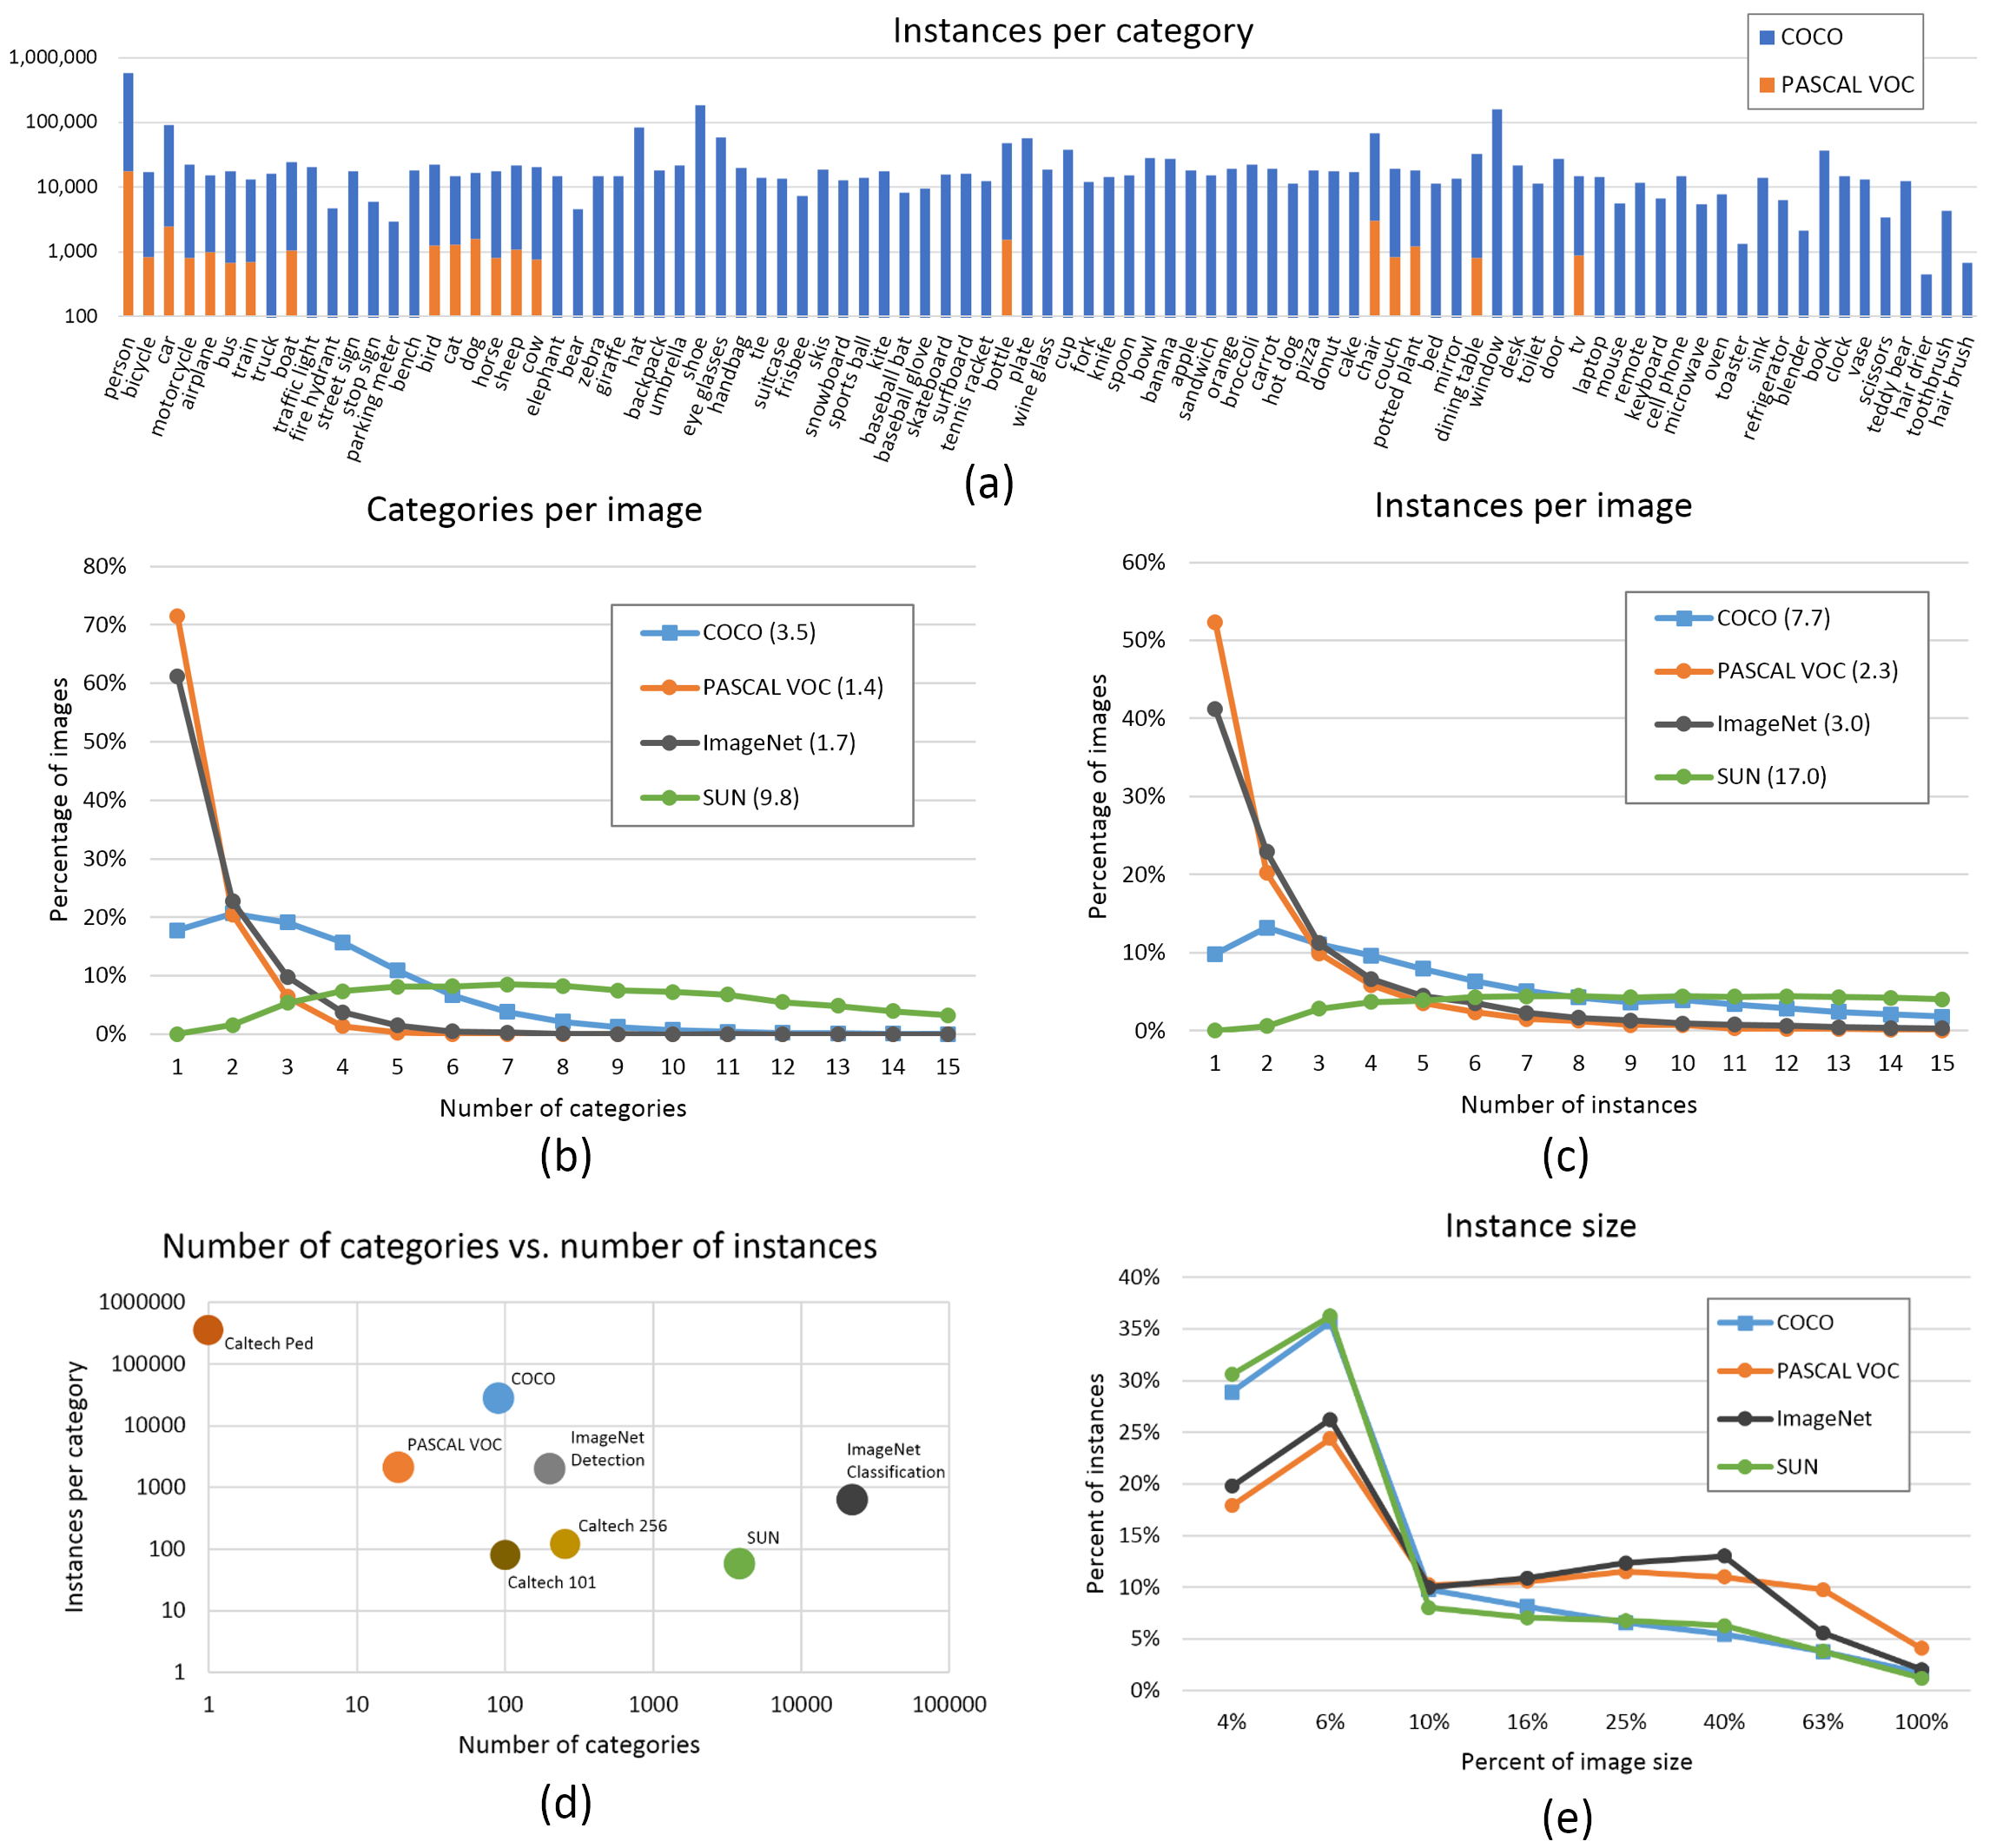
\includegraphics[width=\textwidth]{images/dataanalysis.png}
    \caption{Statistiche riassuntive di \ac{MSCOCO} \cite{lin2014microsoft}}
    \label{fig:dataanalysis_coco}
\end{figure}
\paragraph{Open Images} 
\ac{OID} \cite{krasin2017openimages}, nella versione 5, è un dataset composto da $9.2$ milioni di immagini. Ai giorni d'oggi rappresenta una delle sfide più interessanti insieme a \ac{ILSVRC} e \ac{MSCOCO}. Come per gli altri dataset anche questo si adatta a più task poiché le annotazioni sono state effettuate a livello di singola immagine, di \textit{object detection}, segmentazione e interazioni tra oggetti. 
Analizzando l'aspetto riguardante la rilevazione di oggetti ha ancora più classi rispetto a \ac{ILSVRC} in quanto si arriva a $600$ differenti label su $1.9$ milioni di immagini con \ac{BB} realizzate per la maggiorparte da annotatori professionali interni a Google. In aggiunta i contesti e le ambientazioni in cui sono state catturate le immagini sono molto variegati.
\paragraph{EuroCity}  EuroCity è un dataset proposto da Braun \textit{et al. } nel 2019 \cite{braun2018eurocity}. Le immagini sono state acquisite da un veicolo in movimento in $31$ diverse città europee appartenentei $12$ differenti stati. L'arco temporale attraversa le quattro stagioni, ed anche le condizioni metereologiche, fatta eccezione per forte pioggia e tempeste di neve, sono state tutte acquisite. 

La risoluzione è di $1920 \times 1024$ con un framerate di $20$ immagini al secondo. Una particolarità delle immagini acquisite da queste telecamere è lo spazio colore che arriva a $16$ bit. Quest'alta gamma dinamica si traduce in una più alta qualità dei fotogrammi in condizioni di luce non ottimale, come può essere un controsole o una notturna. 

Per ogni città in media sono state catturate $1.7$ ore di video e le immagini sono state campionate ogni $4$ secondi ($80$ frame). Questo porta ad avere una ripetizione minore di pedoni o oggetti uguali, soprattutto in condizioni trafficate.
Le classi in questo dataset si differenziano in base al veicolo su cui si trovano i pedoni. Sono stati annotati gli esseri umani a piedi, sulle moto, scooter, tricicli, sedie a rotelle e buggy. 
L'occlusione è stata gestita decidendo di annotare l'oggetto nella sua totalità dando una misura spannometrica per le dimensioni della \ac{BB}. 
Riguardo i veicoli invece sono state fatte \ac{BB} separate per il veicolo e la persona al di sopra. 
C'è anche una parte di persone scartate che sono quelle che hanno un'altezza inferiore a 20 pixels. 

\section{Detector basati su metodi tradizionali}
\label{sec:traditional_method}
In questa sezione verranno analizzati in breve i detector più famosi che hanno segnato la storia della \textit{Object Detection} prima dell'avvento del \textit{Deep Learning}.
\paragraph{Viola Jones Detectors}
Nel 2001 P. Viola e M. Jones \cite{viola2001rapid, viola2004robust} sono riusciti a realizzare un modello, chiamato \ac{VJ} Detector, capace di riconoscere volti umani in condizioni non vincolate. L'hardware che fu usato era al passo con i tempi, si parla infatti di un processore Intel Pentium III, ed i risultati erano impressionanti. Molti altri algoritmi di rilevazione di volti infatti giravano decine, se non centinaia, di volte più lenti rispetto ad \ac{VJ} e l'accuratezza era del tutto paragonabile. 

L'approccio usato dai due ricercatori in fase di sviluppo è anche uno dei più basilari, ovvero la finestra scorrevole. Nonostante il compito fosse molto al di la della portata dell'hardware dei tempi questo detector tramite alcune tecniche è riuscito a migliorare drasticamente la sua efficienza in termini di velocità e accuratezza. 
La prima di queste tecniche è un algoritmo chiamato \textit{integral image} che serve a computare efficentemente la somma di valori in un sottoinsieme rettangolare di una griglia. In questo modo si è riusciti a velocizzare le operazioni di filtraggio e convoluzione. 
Il secondo mattoncino con cui è stato costruito \ac{VJ} riguarda la scelta delle feature delle immagini. Le feature venivano estratte grazie alla \textit{Wavelet Haar} ed invece che selezionare manualmente un sottoinsieme di filtri è stato usato Adaboost \cite{freund1999short}. 
Infine la rilevazione veniva effettuata a cascata, in questo modo si riusciva a ridurre lo spreco di risorse evitando di passare più tempo del dovuto su porzioni di immagine dove l'algoritmo aveva una ragionevole certezza fossero sfondo. 
\paragraph{Histogram of Oriented Gradients}
\ac{HOG} è un descrittore di feature per immagini presentato nel 2005 da N. Dalal e B. Triggs \cite{dalal2005histograms}. Il suo scopo era quindi l'estrazione di informazioni utili da un immagine, cercando di scartare il più possibile informazioni inutili. 

La motivazione per la realizzazione è stata la rilevazione di pedoni, tuttavia è facilmente adattabile alla rilevazione di altre classi. 
L'idea dietro queste feature si basa sul gradiente secondo una direzione. Possiamo spiegarlo intuitivamente come la variazione di colore che si ha andando in una determinata direzione di una regione rettangolare dell'immagine. 
L'estrazione procede dividendo l'immagine in celle non disgiunte e per ognuna di esse osservando i pixel che la compongono si calcola un istogramma monodimensionale dei gradienti secondo le varie direzioni. Prendendo tutti gli istogrammi derivanti dalle celle si ottiene una rappresentazione sottoforma di feature \ac{HOG} dell'immagine. In Figura \ref{fig:hog} è possibile vedere un'esempio di estrazione di questo tipo di feature.
\begin{figure}[]
    \centering
    \subfloat[]{
        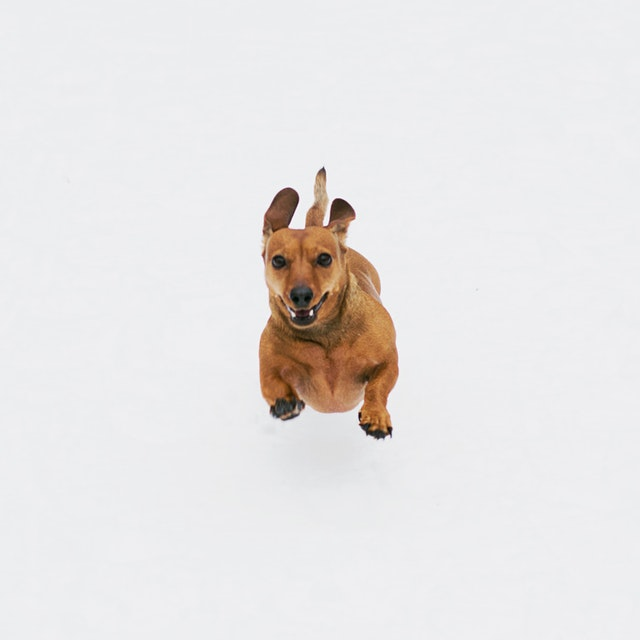
\includegraphics[width=.4\textwidth]{images/dog.jpg}
    }
    \subfloat[]{
        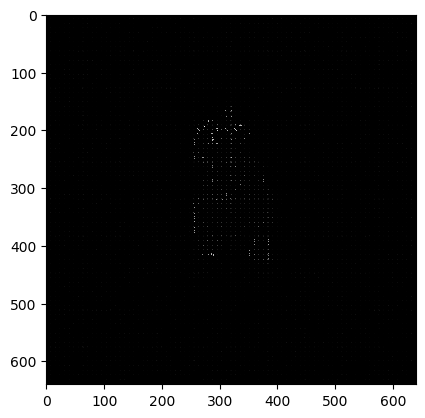
\includegraphics[width=.4\textwidth]{images/dog.png}
    }
    \caption{Esempio di estrazione feature HOG, a sinistra immagine originale, a destra dopo estrazione delle feature} 
    \label{fig:hog} 
\end{figure}

\paragraph{Deformable Part-based Model} 
La realizzazione di \ac{DPM} parte da P. Felzenszwalb nel 2005 come estensione di \ac{HOG} \cite{felzenszwalb2008discriminatively}. Questo detector è di tipo \textit{"Divide et Impera"} in quanto la fase di addestramento può semplicemente essere considerata come l'apprendere la decomposizione di un oggetto in più parti, mentre la fase di inferenza può essere vista intuitivamente come il rilevamento delle parti di un oggetto. 
Successivamente R. Girshick ha esteso questo modello, detto \textit{star-model}, ad un modello mistura \cite{felzenszwalb2010cascade, felzenszwalb2009object, girshick2011object, girshick2012rigid}. In questo modo si è riusciti ad applicare \ac{DPM} a casi reali. Per molti anni è stato considerato un punto di riferimento in quanto vincitore della sfida \ac{VOC} dal 2007 al 2009.

\ac{DPM} è formato da un filtro posizionato alla radice, più tanti altri filtri sottostanti adibiti al riconoscimento delle varie parti che formano un oggetto. Nel modello mistura di Girshick, invece che specificare manualmente cosa dovessero rilevare questi sottofiltri, venivano implementati come variabili latenti e come tali avevano bisogno di una fase di apprendimento supervisionato. 
\section{Detector basati su Deep Learning}
\label{sec:deep_learning_obj}
Come è possibile vedere da Figura \ref{fig:history_object_detection} gli anni tra il $2012$ ed il $2014$ hanno segnato un punto di svolta nella \textit{object detection} grazie a nuovi modelli basati su tecniche di apprendimento profondo. L'era attuale in cui il deep learning ha preso il sopravvento vede una diramazione nelle tecniche sviluppate per la rilevazione degli oggetti, nonostante ciò i due rami sono complementari e sviluppati in parallelo in quanto oggetto di studi recenti. La prima diramazione è quella dei detector \textit{One Stage}, questi detector ottengono prestazioni in inferenza molto elevate, a discapito però di accuratezza e e precisione nella localizzazione più scarse rispetto ai detector \textit{Two Stage}, che però sono più lenti in fase di inferenza. 
\begin{figure}[]
    \centering
    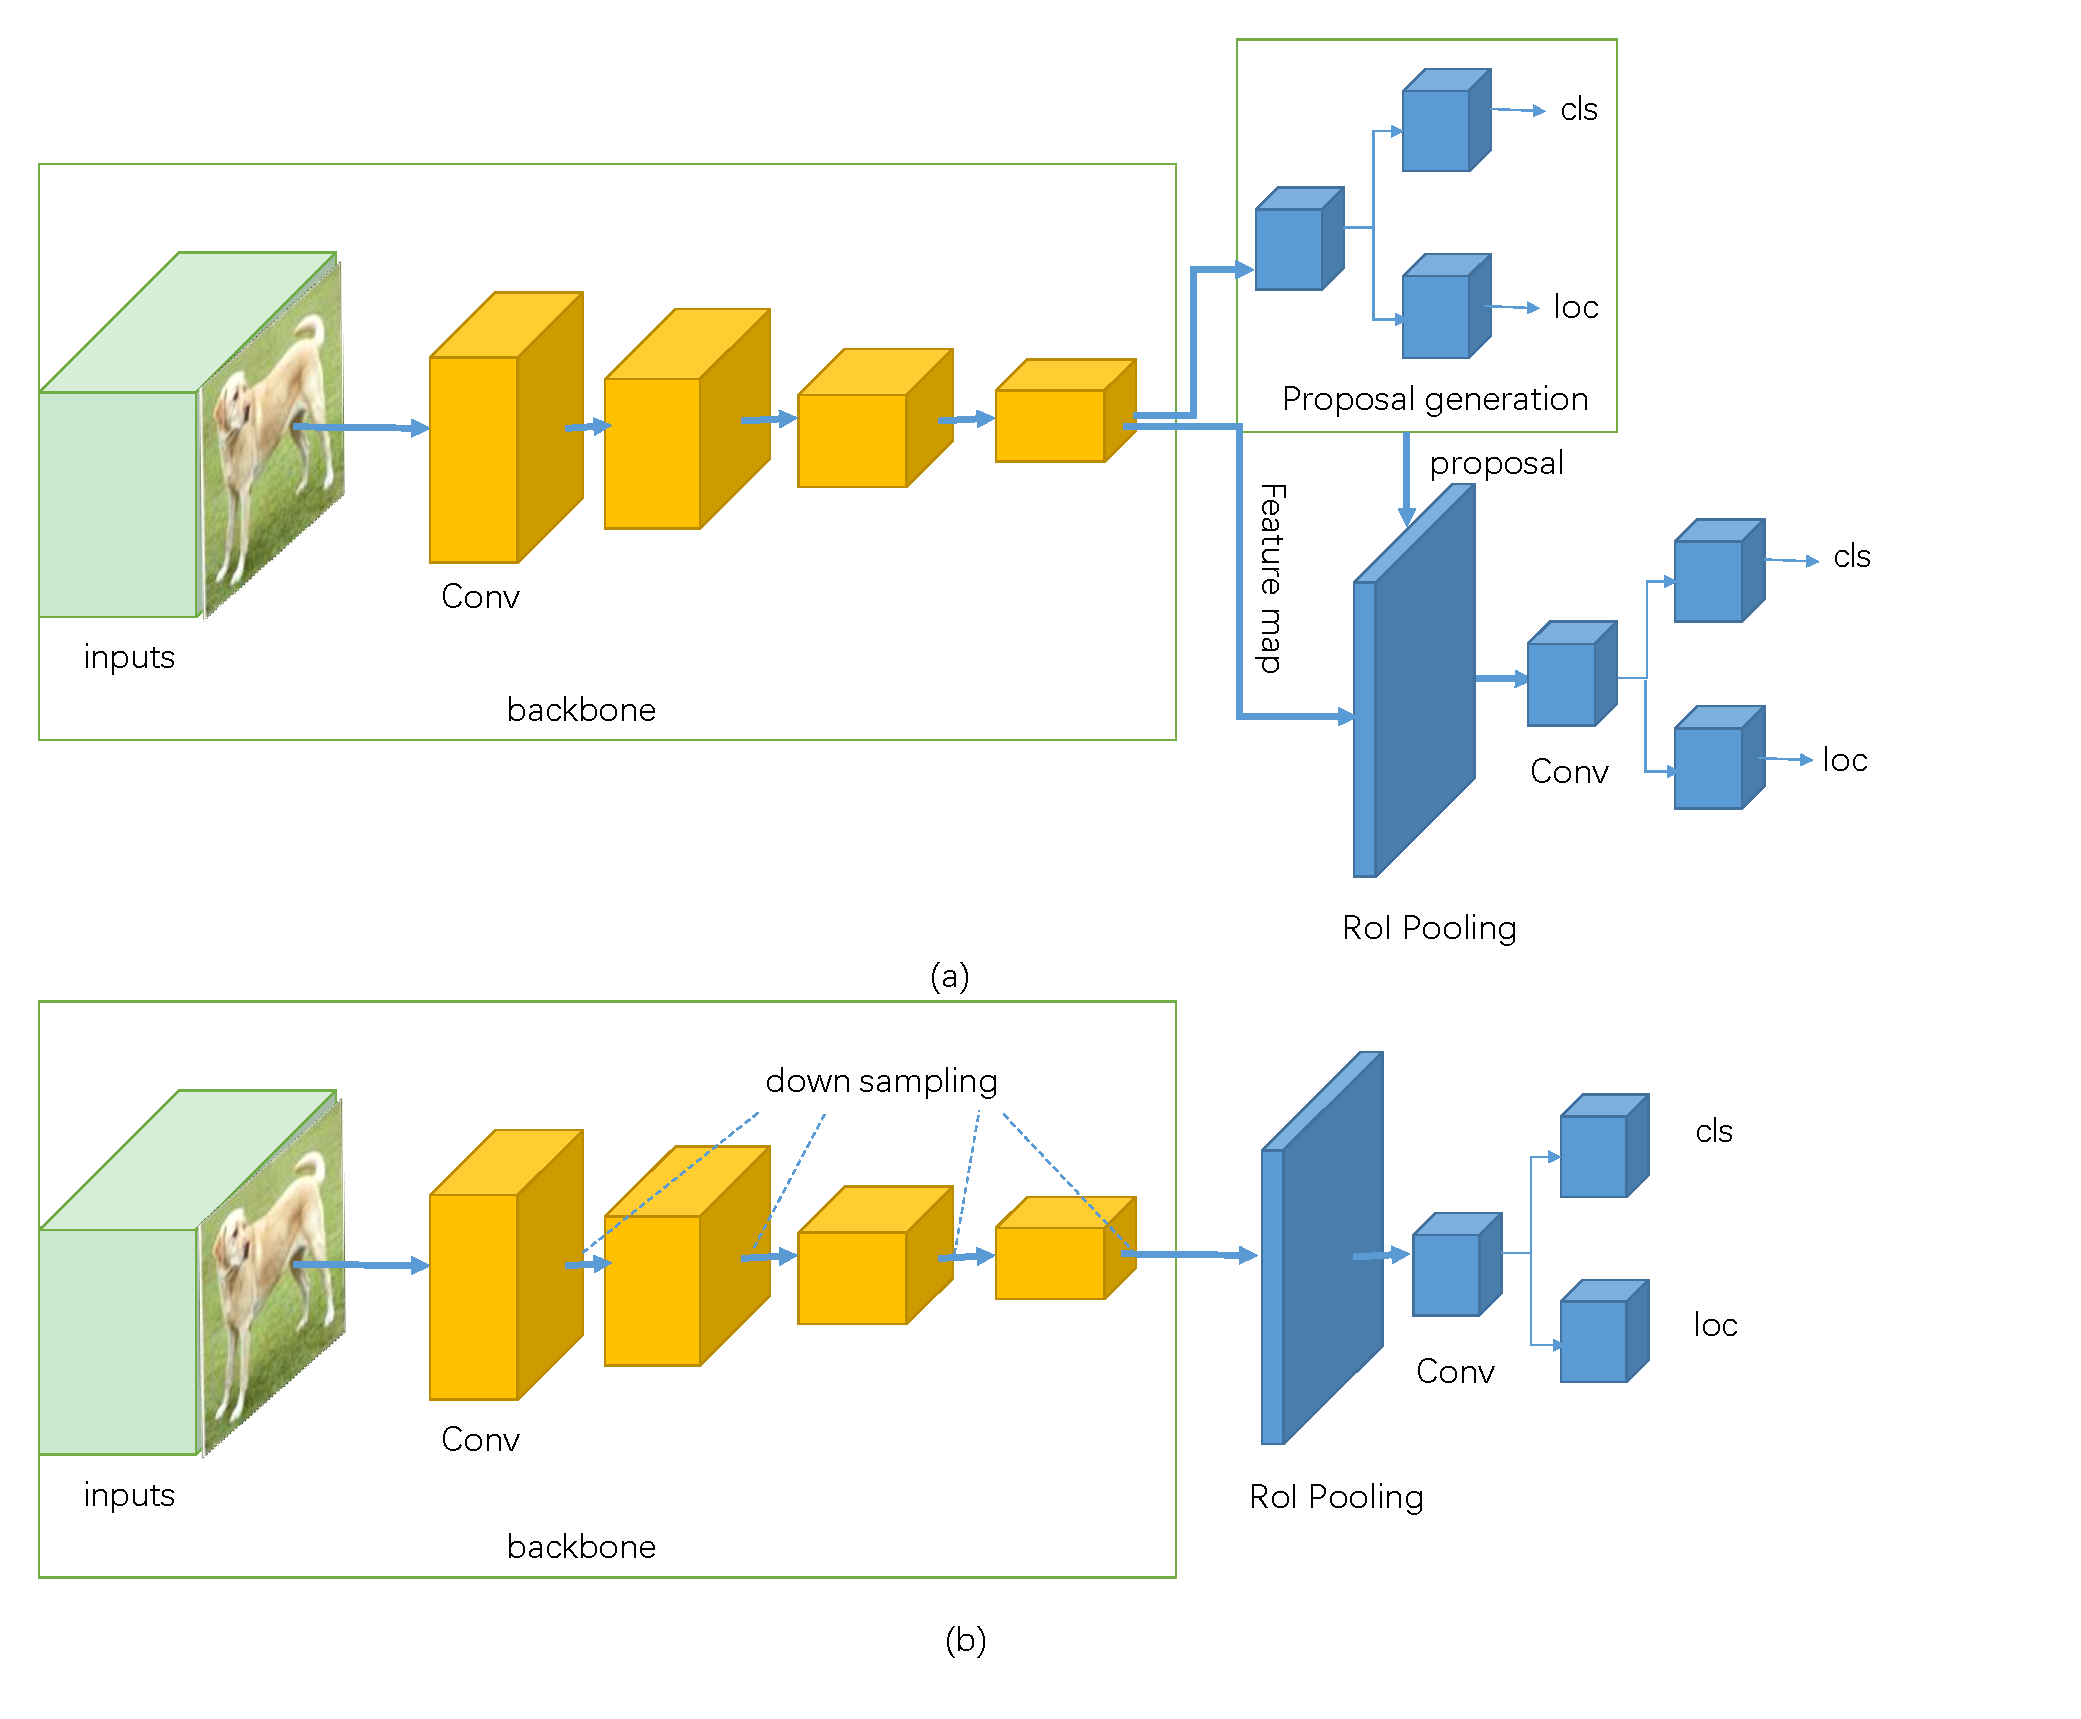
\includegraphics[width=\textwidth]{images/architectures_one_two_stage.pdf}
    \caption{In (a) la struttura di un detector a doppio stadio, in (b) la struttura di un detector a singolo stadio \cite{DBLP:journals/corr/abs-1907-09408}}
    \label{fig:detector_structure}
\end{figure}
\subsection{Estrattori di feature}
\label{sec:feature_extractor}
Nell'era dell'apprendimento profondo anche gli estrattori di feature si sono evoluti. Vengono chiamati in gergo \textit{Backbone Network} e sono reti neurali che prendono in input un'immagine e ne restituiscono le feature che poi andranno in input al modello che si occuperà della rilevazione di oggetti. 

Molte delle reti di backbone usate attualmente sono reti create per la classificazione di immagine, ma senza l'ultimo strato usato come classificatore. Come per molti compiti anche per le estrazioni delle feature possiamo effettuare delle scelte che ci portano ad avere più accuratezza, ma minore velocità di esecuzione o viceversa. 
Reti come ResNet\cite{viola2004robust}, ResNeXt \cite{he2015spatial}, AmoebaNet \cite{girshick2015fast} sono profonde e hanno un elevato grado di connessione tra i vari neuroni, risultano quindi generalmente più accurate, ma conseguentemente avere una struttura così densa porta ad avere effetti negativi sulle prestazioni. 
Molte volte però si può sacrificare un po' di accuratezza per migliorare la velocità, un ambito ad esempio è quello dei dispotivi portatili come possono essere gli smartphone. Reti come MobileNet \cite{ren2015faster}, ShuffleNet \cite{redmon2016you}, Squeezenet \cite{liu2016ssd} o Xception \cite{lin2017feature} sono dei backbone leggeri che possono essere usati per questo scopo. 

\subsection{Two Stage Detector}
\label{subsec:two_stage_detector}
Uno schema basico dell'architettura di un rilevatore a doppio stadio è mostrata in Figura \ref{fig:detector_structure} (a). I cubi gialli sono strati convoluzionali, chiamati blocchi, presenti nella rete di backbone. Essendo nella rete di backbone da questi blocchi si otterà una mappa delle feature, che verrà passata al \ac{ROI} pooling layer per ottenere le feature definitive. 
Le proprietà estratte a quest'ultimo passaggio, nel caso dei detector a doppio stadio, passano generalmente per una \ac{RPN} che propone delle regioni in cui potenzialmente potrebbe essere contenuto un candidato alla rilevazione. L'output della \ac{RPN} a questo punto andrà come input in dei layer convoluzionali aggiuntivi (i cubi blu di Figura \ref{fig:detector_structure}) per la classificazione.
Vedremo qui di seguito alcuni modelli a doppio stadio. 
\paragraph{R-CNN} 
Girshick nel 2014 propone il primo detector a doppio stadio chiamato R-CNN \cite{girshick2014rich}. Il modello è composto da quattro moduli. Il primo modulo genera le cosiddette region proposal, ovvero delle regioni che potenzialmente possono contenere oggetti. Il secondo modulo, partendo da queste regioni genera dei vettori di feature di dimensione fissata (4096 elementi) usando cinque strati convoluzionali e due completamente connessi. Un problema con cui si sono scontrati gli autori in questa fase è stata che l'input di una \ac{CNN} è di dimensione fissata, mentre gli oggetti possono avere dimensioni e proporzioni differenti. È stato quindi fissato l'input della \ac{CNN} come una regione di dimensione $227 \times 227$ e per far combaciare le regioni proposte del primo modulo sono state applicate trasformazioni.
La parte di classificazione è invece appannaggio del terzo modulo, ovvero  un insieme di \ac{SVM}. Le \ac{BB} vengono infine generate tramite regressione dal quarto ed ultimo modulo. Tra le \ac{CNN} i parametri sono condivisi, mentre le \ac{SVM} usate per la classificazione sono totalmente indipendenti l'una dall'altra.

La fase di addestramento di R-CNN si fa su ogni singolo componente in maniera separata. Come prima cosa viene realizzata una fase di pre-addestramento, seguita da una fase di addestramento fine. Dopodiché si vanno ad addestrare in maniera separata i classificatori \ac{SVM} e gli strati di regressione per generare le \ac{BB}.
Riguardo la classificazione un aspetto interessante di cui tenere conto è l'applicazione della \ac{IoU} o indice di Jaccard, ovvero un valore che indica la sovrapposizione tra due regioni. Varia tra 0 e 1, con 0 quando non c'è alcuna sovrapposizione ed 1 quando la sovrapposizione è totale. La \ac{IoU} si calcola prendendo in considerazione la \ac{BB} \textit{vera} e la \ac{BB} predetta in fase di inferenza. In particolare è definita come il rapporto tra l'area di intersezione delle due regioni e l'unione delle due aree. 

\paragraph{Spatial Pyramid Pooling Networks} In R-CNN uno dei problemi era nel secondo modulo quando le \ac{CNN} richiedevano un input di dimensione fissata. Con \ac{SPPNet} \cite{he2015spatial} si risolve il problema introducendo un layer di pooling piramidale che permette alle \ac{CNN} di lavorare anche con input di dimensione differente, senza necessità di applicare trasformazioni alla regione. In Figura \ref{fig:spnnet_structure} possiamo vedere come è stato realizzato questo nuovo layer di pooling piramidale. 

Con l'uso di questo nuovo strato le feature possono essere estratte solamente una volta e dall'intera immagine, il che porta \ac{SPPNet} ad essere circa 20 volte più veloce di R-CNN, senza perdere in accuratezza. 
Nonostante ciò sono presenti lo stesso alcune problematiche infatti come per R-CNN la fase di addestramento è ancora realizzata in più passaggi.
\begin{figure}[]
    \centering
    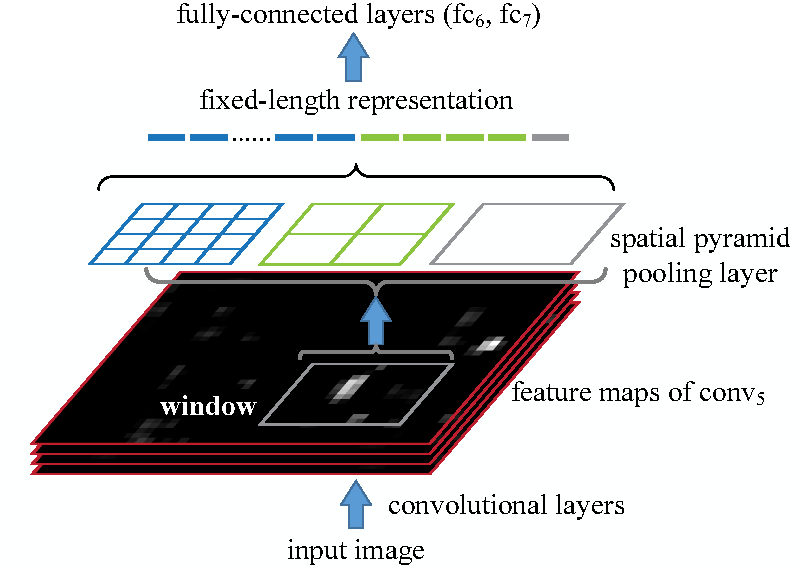
\includegraphics[width=0.7\textwidth]{images/spm_det.pdf}
    \caption{Struttura di \ac{SPPNet} \cite{he2015spatial}}
    \label{fig:spnnet_structure}
\end{figure}
\paragraph{Fast R-CNN}
Fast R-CNN, proposta sempre da R. Girshick, \cite{girshick2015fast} è una versione migliorata di R-CNN. Uno dei grandi difetti di R-CNN era la velocità in quanto per ogni regione candidata era necessario un passaggio sulle \ac{CNN} per estrarre le feature. 
Con Fast R-CNN le feature vengono estratte in un unico momento e dall'intera immagine e successivamente passate ad  un \ac{ROI} pooling layer che restituisce in uscita vettori di dimensione fissata da passare agli strati di classificazione e regressione. 
A differenza di R-CNN e \ac{SPPNet} l'addestramento è composto da una sola fase, e questo è reso possibile da una misura di loss comune a tutta la struttura. 
Un altro miglioramento rispetto a R-CNN, e che accomuna questo detector a \ac{SPPNet}, è che vengono preservate le informazioni spaziali delle regioni candidate in quanto non c'è più necessità di avere input di dimensione fissa per le \ac{CNN}. 

Tramite queste migliorie si ottengono vantaggi notevoli rispetto a R-CNN, sia in fase di training che di inferenza. In addestramento si ha uno speedup di circa 9 volte, mentre si ha un incremento di prestazioni in fase di inferenza che arriva fino a 223 volte. 
\paragraph{Faster R-CNN}
Tre mesi dopo la presentazione di Fast R-CNN venne presentata un'ulteriore versione migliorata chiamata Faster R-CNN \cite{ren2015faster}. Il collo di bottiglia di Fast R-CNN è la generazione delle regioni candidate a contenere oggetti. Con Faster R-CNN viene risolto con l'utilizzo di una \ac{RPN}, ovvero una rete convoluzionale in grado di generare efficentemente regioni di diverse dimensioni e proporzioni. Viene quindi scartata la parte iniziale di Fast R-CNN e sostituita con questa nuova \ac{RPN} che in poche parole dice a Fast R-CNN \textit{dove guardare}.

L'input di una \ac{RPN} è un'intera immagine e l'ouput sono regioni rettangolari con un indice di appartenza ad una determinata classe. 
In più in Faster R-CNN, grazie all'implementazione di una \ac{RPN}, vengono utilizzate anche le \textit{Anchor Boxes} che semplificano la rilevazione di oggetti con dimensioni differenti. 
\paragraph{FPN}
Nel 2017 Lin \textit{et al.} hanno proposto \ac{FPN} \cite{lin2017feature} sulla base di Faster R-CNN. Prima di \ac{FPN} l'idea era di eseguire la rilevazione di oggetti basandosi solamente sull'output dell'ultimo livello dell'estrattore di feature. Tuttavia però alcune informazioni contenute nei layer più profondi della \ac{CNN} possono essere utili, per questo motivo è stata fatta un'architettura top down con connessioni laterali sfruttando la piramidalità intrinseca delle \ac{CNN}. Ora \ac{FPN} è utilizzato in molti modelli, tra cui anche RetinaNet. 
\subsection{One Stage Detector}
\label{subsec:one_stage_detector}
Lo schema architetturale di un detector a singolo stadio è visibile in Figura \ref{fig:detector_structure} (b). Inizialmente è sempre presente un backbone che servirà ad estrarre le feature dall'immagine in input, però a differenza di \ref{subsec:two_stage_detector} non è più presente una eventuale \ac{RPN}, bensì dal \ac{ROI} pooling layer si passa direttamente a dei layer convoluzionali che si occuperanno di rilevare e classificare l'oggetto di interesse. 

Come detto all'inizio della Sezione \ref{sec:deep_learning_obj} la struttura dei modelli a singolo stadio li porta ad avere una accuratezza ed una precisione nella localizzazione minore rispetto alla controparte a doppio stadio. Una struttura più semplice dal punto di vista degli strati però porta ad avere maggiore velocità di elaborazione. Di seguito vedremo alcuni dei più famosi modelli a singolo stadio. In particolare in Sezione \ref{sec:retinanet} vedremo in dettaglio RetinaNet, ovvero la rete neurale usata durante il lavoro di ricerca di questa tesi.  
\paragraph{YOLO}
Redmon \textit{et al.} proposero un nuovo detector chiamato \ac{YOLO} con lo scopo di effettuare rilevazioni in tempo reale su video tratti da webcam \cite{redmon2016you}. 
Il flusso di \ac{YOLO} inizialmente prevede la divisione dell'immagine in input tramite una griglia di dimensione $S \times S$. 
Ogni elemento della griglia è responsabile di predirre $B$ \ac{BB} ed i loro punteggi di confidenza. Questo punteggio viene calcolato per rispecchiare la confidenza che ha il modello nell'affermare che una certa \ac{BB} contenga un oggetto e per affermare anche quanto è precisa questa predizione. Viene infatti calcolato come $Pr(Oggetto) * IOU^{thruth}_{pred}$.
Quindi la struttura di una \ac{BB} è rappresentabile come una quintupla $(x, y, w, h, confidenza)$ dove i primi quattro valori rappresentano le coordinate nello spazio, e l'ultimo la confidenza. 
Il singolo elemento della griglia inoltre calcola un vettore $C$ dimensionale che rappresenta la probabilità condizionale $P(Classe | Oggetto)$ per ogni classe. In Figura \ref{fig:yolo_structure} è possibile vedere come è strutturata la rete nella sua totalità. 
\begin{figure}[]
    \centering
    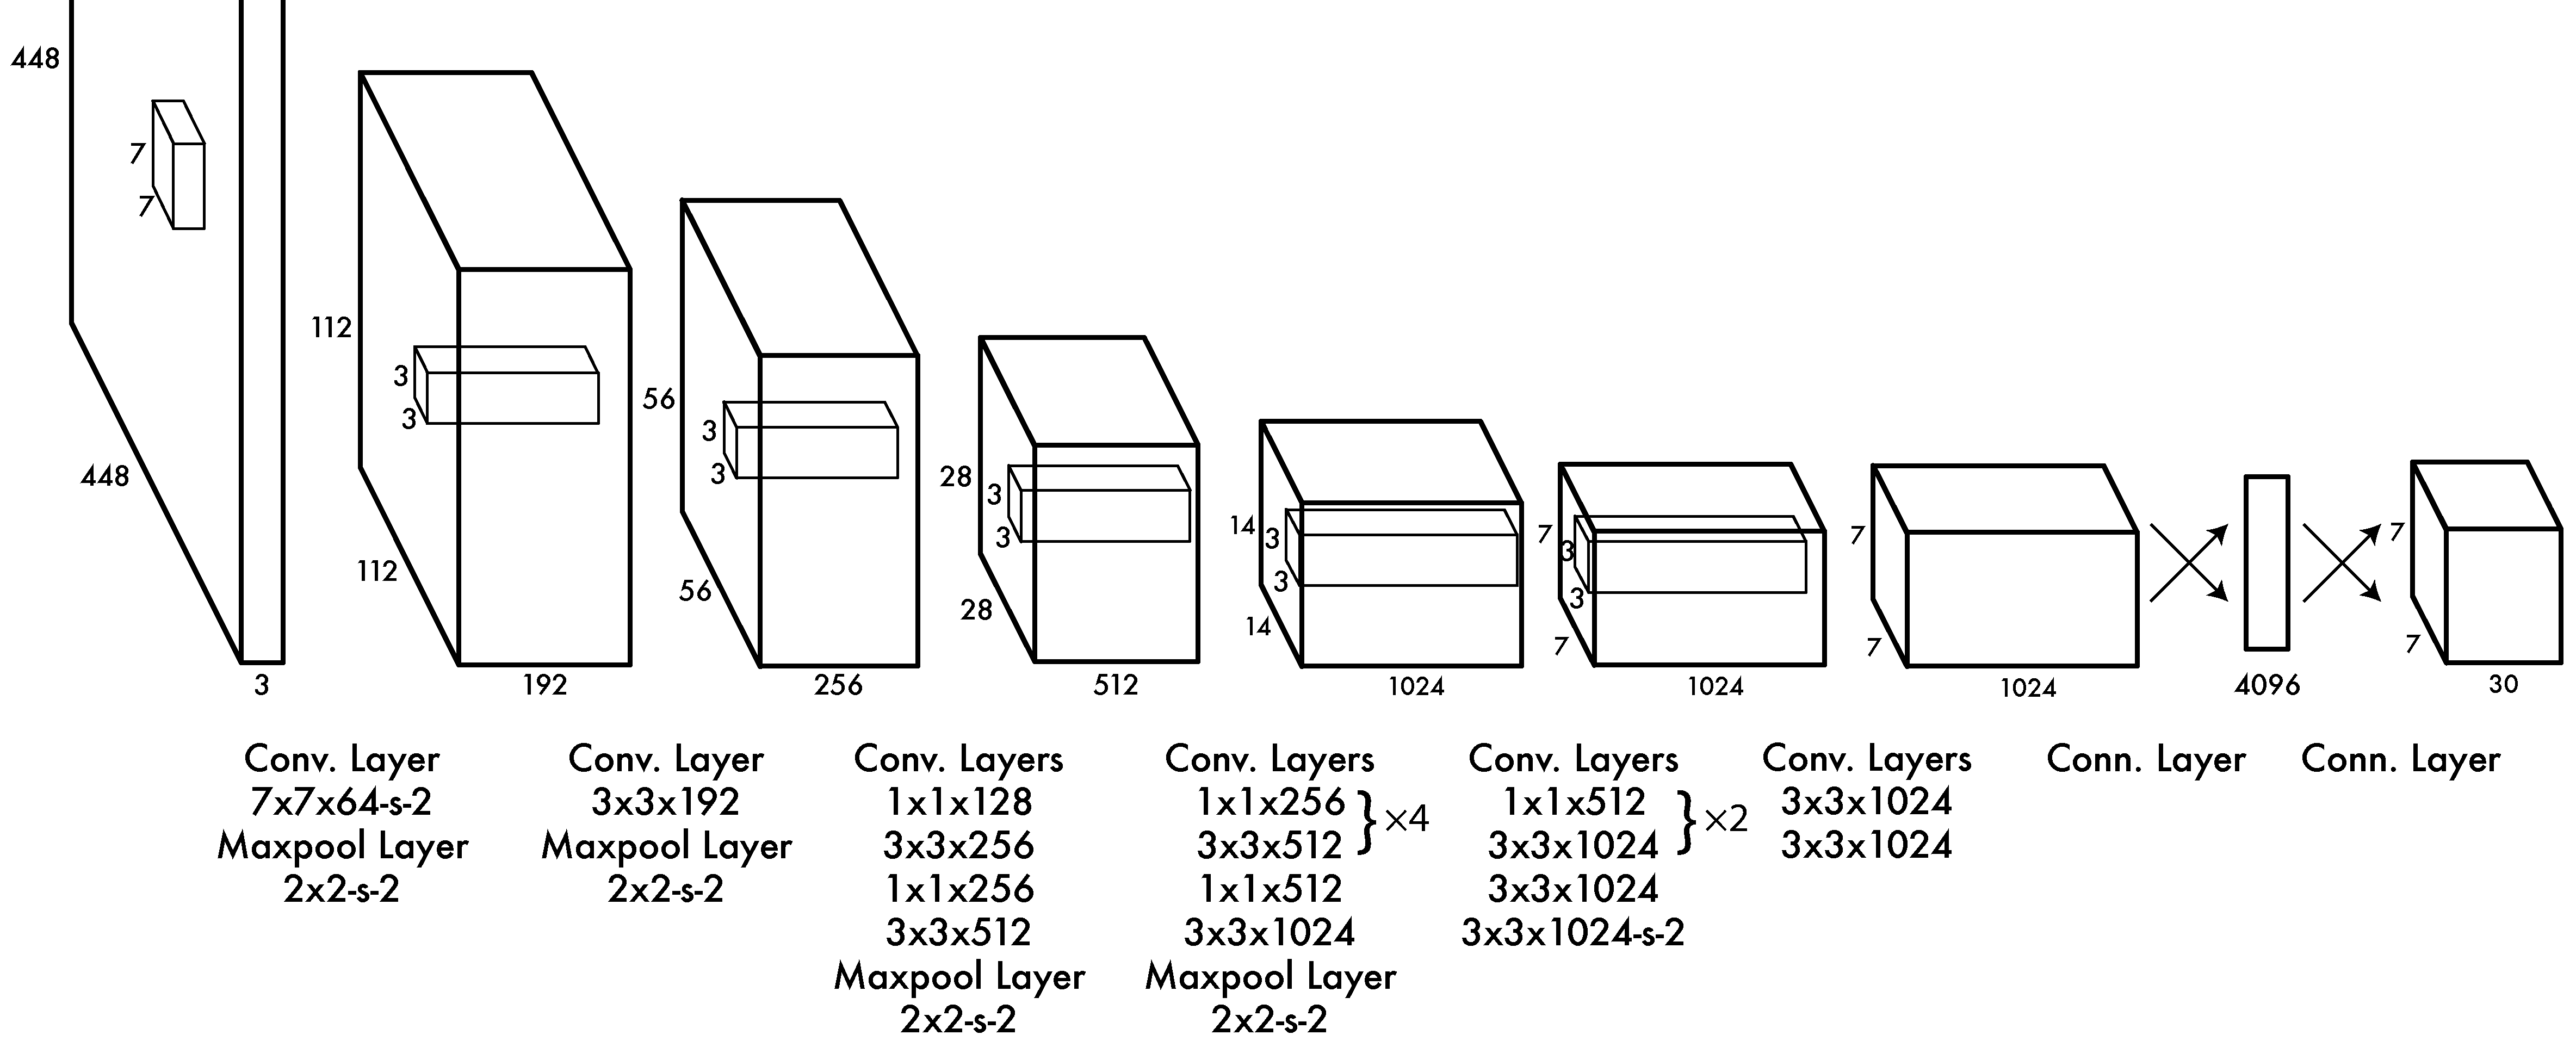
\includegraphics[width=\textwidth]{images/net_yolo.pdf}
    \caption{Struttura di \ac{YOLO} \cite{redmon2016you}}
    \label{fig:yolo_structure}
\end{figure}
\paragraph{YOLO V2}
\ac{YOLO} V2 come intuibile dal nome è la seconda versione del detector \ac{YOLO} che lo migliora in alcuni aspetti utilizzando tecniche prese da lavori precendenti \cite{redmon2017yolo9000}.
Innanzitutto è stata adottata la \textit{Batch Normalization} davanti ad ogni layer convoluzionale \cite{ioffe2015batch}. Questi strati di regolarizzazione favoriscono la fase 
di training rendendola più veloce. Inoltre si ottiene un miglioramento del $2\%$ sulla \ac{map}.
Il secondo miglioramento è stato aumentare la risoluzione dell'input del classificatore. Nella prima versione la risoluzione è di $224 \times 224$, che viene incrementata $448 \times 448$ quando si effettua la rilevazione.
In \ac{YOLO} V2 viene prima effettuato un fine tuning di 10 epoche del classificatore usando come risoluzione $448 \times 448$.
La prima versione di \ac{YOLO} per predirre la posizione delle \ac{BB} usava degli strati totalmente connessi posizionati dopo i layer convoluzionali. Ora invece in \ac{YOLO} V2 viene usato l'approccio delle \textit{Anchor Boxes} rimuovendo quindi questi ultimi layer insieme al layer di pooling. 
In questo modo si mantiene una feature map ad alta risoluzione adatta allo scopo. È stata modificata anche la rete per far si che operi alla risoluzione di $416 \times 416$. Il numero $416$ è stato scelto per via del fatto che si possa mappare con feature $13 \times 13$, ed avendo un numero di pixel dispari si ha un unico pixel centrale. 

Le predizioni riguardanti dimensioni e proporzioni delle \ac{BB} fino ad ora veniva fatto in maniera empirica, anche in detector come Fast R-CNN. La seconda versione di \ac{YOLO} usa l'algoritmo di clustering \textit{K-Means} sull'insieme dei dati per l'addestramento per ottenere delle buone probabilità a priori.  La particolarità è che non viene usata la distanza euclidea, ma una misura basata sull'\ac{IoU}. 
Un altro aspetto migliorato riguarda le feature. L'estrazione come detto in precedenza prevede finestre più piccole di dimensione $13 \times 13$, questo porta ad un miglioramento nella rilevazione di oggetti piccoli. È presente anche un layer che concatena feature a dimensione $26 \times 26$ con quelle a $13 \times 13$ su canali differenti. 
Il training ora viene fatto usando una risoluzione di input differente che varia di 10 batch in 10 batch. Il modello effettua una riduzione di un fattore $32$ dalla risoluzione standard di $416 \times 416$ ad una feature map di dimensione $13 \times 13$. Per mantenere questa strutura quindi la risoluzione di input varia da minimo di $320 \times 320$ fino ad un massimo di $608 \times 608$ attraversando esclusivamente i multipli di $32$. Da \ac{YOLO} V2 deriva anche \ac{YOLO} 9000 che riesce a rilevare, a discapito di un degrado delle performance, fino a 9000 oggetti.
\paragraph{YOLO V3} 
\ac{YOLO} V3 è l'ultima versione, ed ottenuta  tramite miglioramenti dalla V2 \cite{redmon2018yolov3}. La prima miglioria effettuata è sulla predizione dei label, in \ac{YOLO} V3 è possibile assegnare ad una \ac{BB} più classi. Non si usa più un classificatore \textit{softmax}, bensì un classificatore logistico coadiuvato dalla loss \textit{cross-entropy}.

All'estrattore di feature sono stati aggiunti alcuni layer convoluzionali che permettono di predirre \ac{BB} con 3 scale differenti. L'ultimo di questi layer restituisce in output un tensore 3d che rappresenta la predizione in termini di coordinate della \ac{BB}, misura di confidenza e predizioni delle classi. Gli esperimenti effettuati dagli autori sono stati fatti sul dataset \ac{MSCOCO} e sono state predette 3 \ac{BB} ad ogni scala differente, perciò il tensore di output è di dimensione $N \times N \times [3 \cdot (4 + 1 + 80)]$, dove l'ultima dimensione è strutturata in questo modo in quanto le scale sono 3 differenti, per ogni \ac{BB} ci sono 4 coordinate, più 1 misura di confidenza, più $80$ valori di probabilità sulle classi. 
Terza novità è la rete di backbone, che cambia passando a \textit{Darknet-53}
\paragraph{SSD} 
\ac{SSD} \cite{liu2016ssd} è detector basato su una rete neurale convoluzionale che produce un insieme di dimensione fissata composto da \ac{BB} e indici di confidenza per indicare la presenza o meno di oggetti al loro interno. Infine è presente una fase di \ac{NMS} per produrre le rilevazioni finali. 

La rete è divisa fondamentalmente in due parti, la parte iniziale è un'architettura standard usata per la classificazione di immagini ma troncata in fondo in maniera da rimuovere gli ultimi layer che si usano per la classificazione. Successivamente è presente una struttura ausiliaria che si divide a sua volta in altre tre fasi:
\begin{itemize}
    \item Feature multi scala: alla fine della rete troncata vengono aggiunti una serie di layer convoluzionali che via via diminuiscono in dimensione e perciò permettono di effettuare rilevazioni su scale multiple. 
    \item Predittori convoluzionali: Ogni layer aggiunto alla fase precedente produce un insieme fisso di predizioni usando un gruppo di filtri convoluzionali. Considerando un layer con dimensione $m \times n$ a $p$ canali abbiamo un filtro di dimensione $3 \times 3 \times p$.
    \item \ac{BB} di default: è un approccio simile a quanto già visto con le \textit{Anchor Boxes}, tuttavia sono applicate a diverse mappe di feature a diverse risoluzioni. 
\end{itemize}
Durante l'addestramento di \ac{SSD} si cerca di far combaciare il più possibile le \ac{BB} di default con le \ac{BB} che rappresentano la \textit{ground truth}. Per fare ciò bisogna determinare quale \ac{BB} di default ha maggior intersezione con le \ac{BB} rappresentanti la verità. Questo si fa attraverso l'indice di Jaccard (o \ac{IoU}) e prendendo quelle \ac{BB} di default con gli indici maggiori. 
Dopo questa fase di matching delle \ac{BB} ci sono molte predizioni negativi che introducono sbilanciamento tra esempi positivi e negativi in fase di training, perciò si adotta una tecnica di \ac{HNM} ordinando gli esempi negativi secondo il loro livello di confidenza e prendendo solo i più alti. In questo modo si riesce a ridurre il rapporto tra esempi negativi e positivi a circa 3 su 1.
\paragraph{Deconvolutional SSD} 
\ac{DSSD} \cite{fu2017dssd} è una versione modificata di \ac{SSD} che aggiunge un modulo di predizione e di deconvoluzione, oltre ad usare ResNet-101 come backbone. In Figura \ref{fig:ssd_architectures} è possibile vedere un confronto delle due architetture.
\begin{figure}
    \centering
    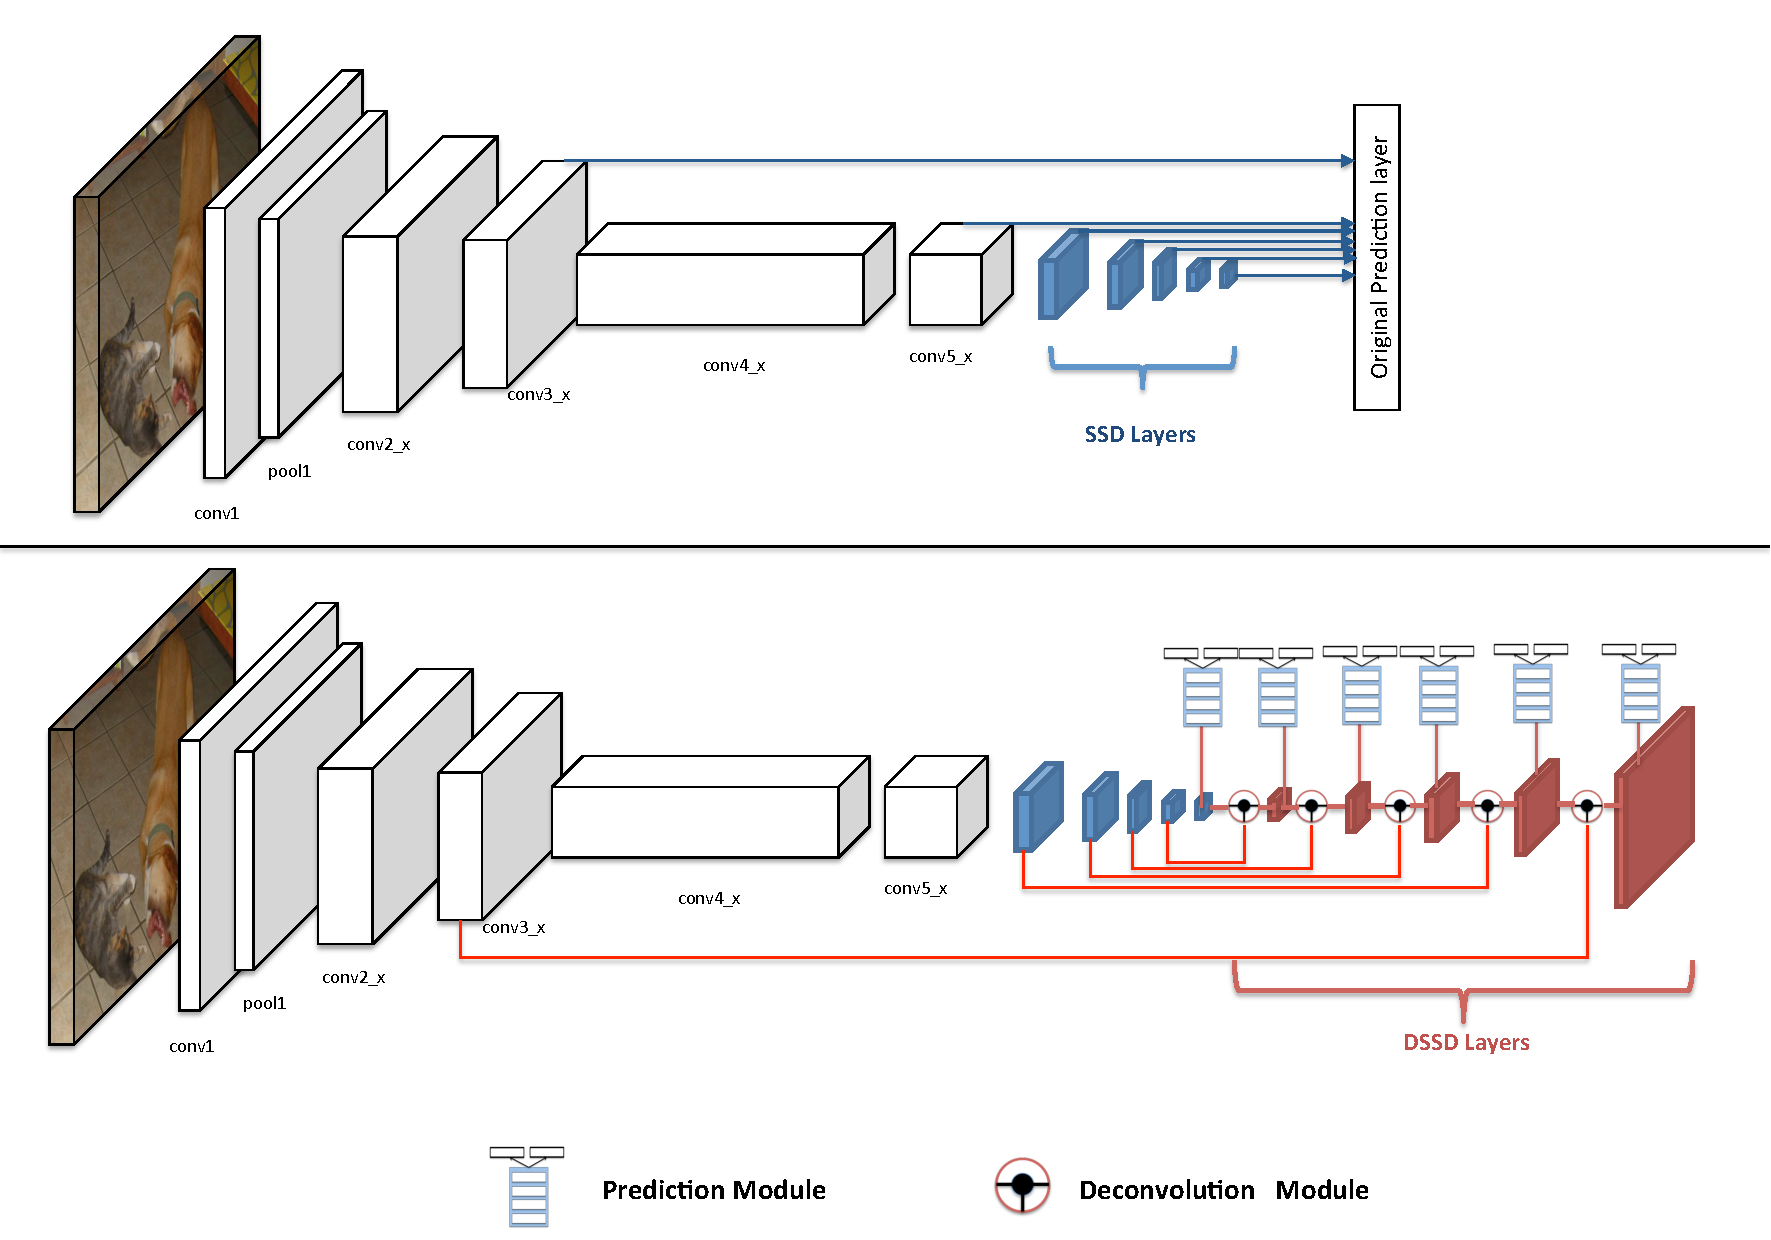
\includegraphics[width=0.8\textwidth]{images/architecture_ssd.pdf}
    \caption{Architetture di SSD e DSSD. In blu i layer di SSD, in rosso quelli di DSSD.}
    \label{fig:ssd_architectures}
\end{figure}

I moduli di predizione aggiunti via via nel corso della computazione servono a rilevare oggetti di varie dimensioni e proporzioni, mentre i layer di deconvoluzione portano ad avere delle feature più rappresentative.
\paragraph{M2DET} \cite{zhao2019m2det}
Nasce per andare incontro all'esigenza di rilevare oggetti uguali, ma con dimensioni differenti. Come si può vedere in Figura \ref{fig:m2det_architectures} dopo la rete di backbone per l'estrazione delle feature è presente una \ac{MLFPN} composta a sua volta di tre moduli:
\begin{itemize}
    \item \ac{FFM}: serve ad fondere le feature provenienti da livelli diversi, usano layer convoluzionali di dimensione $1 \times 1$ per comprimere i canali di input e aggregare le feature map. 
    \item \ac{TUM}: genera un gruppo di feature multi scala. È formato da una serie di layer convoluzionali di dimensione $3 \times 3$ con stride $2$. 
    \item \ac{SFAM}: aggrega le feature generate da \ac{TUM} in strutture piramidali tramite concatenazione.
\end{itemize}
\begin{figure}
    \centering
    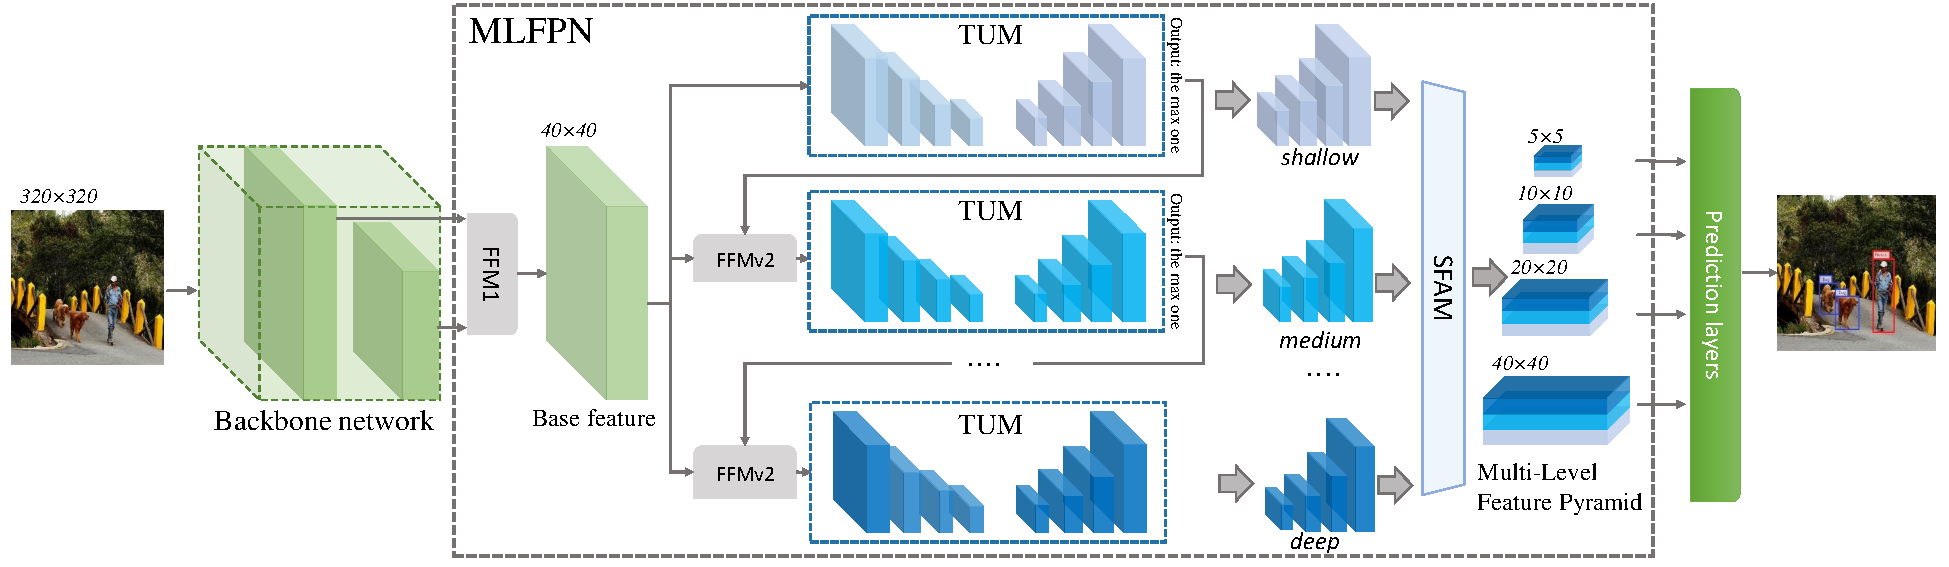
\includegraphics[width=\textwidth]{images/pipeline_m2det.pdf}
    \caption{Struttura di m2det \cite{zhao2019m2det}}
    \label{fig:m2det_architectures}
\end{figure}

\section{RetinaNet}
\label{sec:retinanet}
Il trade-off tra precisione e velocità è sempre stato un punto cruciale che ha determinato la scelta tra detector a singolo stadio ed a doppio stadio. Con RetinaNet \cite{lin2017focal} si tenta di risolvere questo problema. Secondo i ricercatori è da imputare al forte sbilanciamento che si incontra in fase di training tra esempi di sfondo ed esempi di oggetti. Quindi è stata introdotta una versione modificata della classica \textit{cross-entropy} loss chiamata \textit{Focal Loss} che migliora la situazione. 
\subsection{Focal Loss}
\label{subsec:focal_loss}
Prima di introdurre la \textit{Focal Loss} è necessario ricordare la forma della \textit{Cross-Entropy} per problemi di classificazione binaria:
$$\textrm{CE}(p,y) = \begin{cases} -\log(p) &\text{se $y = 1$}\\
-\log (1 - p) &\text{altrimenti.}\end{cases}$$ con $y \in \{\pm 1 \}$ che specifica la classe di \textit{ground truth} e $p$ valore di probabilità per la classe con $y=1$.
Per comodità si definisce un'indice $p_t$ che indica se un esempio è classificato bene o meno:
$$p_t = \begin{cases} p &\text{se $y = 1$}\\ 1 - p &\text{altrimenti,}\end{cases}$$
un valore di $p_t$ superiore a $0.5$ indica che l'esempio è stato classificato correttamente, viceversa indica un errore nella classificazione. Con $p_t$ è poi possibile riscrivere $\textrm{CE}(p, y) = \textrm{CE}(p_t) = -log(p_t)$. In Figura \ref{fig:focal_loss} la curva blu rappresenta la \textit{Cross Entropy} ed è possibile notare una proprietà riguardante gli esempi considerati facili da classificare, ovvero quelli con un valore $p_t$ molto superiore a 0.5. Come è possibile vedere la loss di questi esempi ha comunque un valore elevato, nonostante siano considerati facili. Quindi sommando questa serie di valori si ottiene una loss comunque alta che non permette di concentrarsi sull'addestramento degli esempi considerati positivi e dare minor peso agli esempi negativi quali lo sfondo. 
\begin{figure}
    \centering
    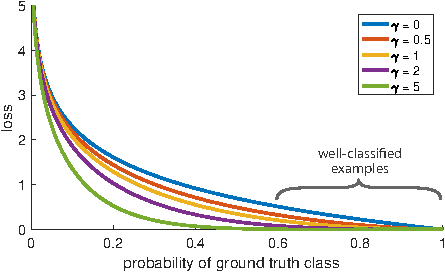
\includegraphics[width=0.8\textwidth]{images/loss.pdf}
    \caption{Focal Loss al variare di $\gamma$}
    \label{fig:focal_loss}
\end{figure}
Questo forte sbilanciamento tra sfondo e oggetti è di circa $1$ a $10000$ e per evitare effetti disastrosi sulla funzione di loss i ricercatori hanno cercato innanzitutto di bilanciare la \textit{Cross Entropy} con un fattore $\alpha \in [0, 1]$ per la classe $1$ e $1 - \alpha$ per la classe $-1$. Per comodità, analogamente a $p_t$ è possibile definire anche $\alpha_t$ come:
$$\alpha_t = \begin{cases} \alpha &\text{se $y = 1$} \\ 1 - \alpha &\text{altrimenti}\end{cases}$$ 
Quindi partendo da $\alpha_t$ è possibile definire la nuova \textit{Cross Entropy} bilanciata $\textrm{CE}_b(p_t)=-\alpha_t log(p_t)$. 

Con il termine $\alpha$ si è riusciti quindi a bilanciare gli esempi negativi da quelli positivi, però rimane il problema di bilanciare tra esempi la cui detection è facile o difficile, ovvero quelli per cui abbiamo un valore $p_t$ elevato o basso. Lo scopo quindi è dare poca rilevanza agli esempi facilmente classificabili e molta rilevanza a quelli difficilmente classificabili. Si aggiunge quindi alla \textit{Cross Entropy} un nuovo termine $(1-p_t)^\gamma$ con $\gamma \geq 0$ ottenendo una nuova funzione di loss detta \textit{Focal Loss}:
$$\textrm{FL}(p_t) = -(1-p_t)^\gamma log(p_t)$$.
Realizzando un'analisi di questa funzione possiamo affermare che avendo un esempio classificato male ($p_t < 0.5$), il fattore modulativo $(1-p_t)^\gamma$ è vicino a $1$ e la loss rimane più o meno invariata, mentre più $p_t$ tende ad $1$ e più il fattore modulativo sarà vicino a $0$, rendendo così la loss per gli esempi classificati bene meno efficace.
Possiamo inoltre immaginare $\gamma$ come un parametro che permette di gestire questa riduzione di efficacia. Ponendo $\gamma = 0$ ci si riconduce alla \textit{Cross Entropy}, mentre più si aumenta e più si ottiene la riduzione di efficacia per gli esempi classificati bene. 

Unendo la \textit{Focal Loss} e la \textit{Cross Entropy} loss bilanciata si ottiene la forma di \textit{Focal Loss} utilizzata all'interno di RetinaNet:
$$\textrm{FL}(p_t) = \alpha_t(1-p_t)^\gamma log(p_t)$$
\subsection{Struttura del detector}
\label{subsec:retinanet_structure}
RetinaNet è composta da tre sottoreti, la prima è il backbone, le altre due sono una rete convoluzionale adibita alla classificazione e l'ultima una rete convoluzionale per la regressione sulle \ac{BB}. In Figura \ref{fig:retinanet_structure} è possibile vedere questa struttura appena descritta.
\begin{figure}
    \centering
    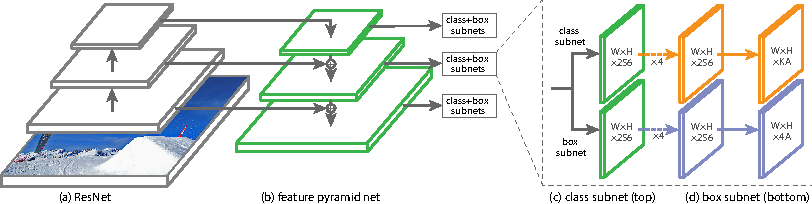
\includegraphics[width=\textwidth]{images/retinanet_net.pdf}
    \caption{Struttura di RetinaNet}
    \label{fig:retinanet_structure}
\end{figure}
Descriveremo di seguito le componenti del modello.
\paragraph{Feature Pyramid Network Backbone}
Una parte del backbone di RetinaNet è una \ac{FPN} \cite{lin2017feature} che costruisce una struttura di feature piramidali a partire da un'immagine in input. Ogni livello della piramide può essere utilizzato per rilevare oggetti con dimensioni differenti. 
La \ac{FPN} utilizzata è stata costruita al di sopra di una architettura ResNet \cite{he2016deep}. È stata quindi costruita una struttura prendendo i livelli che vanno da $P_3$ a $P_7$ tale per cui il livello $P_l$ con $l \in [3, 7]$ ha una risoluzione minore di un fattore $2^l$ rispetto all'input. Tutti i livelli hanno $C=256$ canali. Inoltre a differenza di \cite{lin2017feature} i livelli che vanno da $P_3$ a $P_5$ sono calcolati direttamente a partire dai corrispondenti livelli $C_3, C_4$ e $C_5$ di ResNet. Riguardo $P_6$ è ottenuto tramite un layer convoluzionale con filtri $3 \times 3$ e stride $2$ da $C_5$. $P_7$ è ottenuto applicando ReLU alla stessa operazione effettuata per ottenere $P_6$, ma applicata su $C_6$.
\paragraph{Anchor}
Le \textit{Anchor Boxes} sono simili a quelle utilizzate in \cite{lin2017feature}. Hanno un'area che può variare da $32 \times 32$ a $512 \times 512$ rispettivamente sui livelli della piramide delle feature che vanno da $P_3$ a $P_7$. Come in \cite{lin2017feature} ogni livello della piramide usa \textit{Anchor Boxes} di tre differenti proporzioni ($1:2, 1:1, 2:1$). Inoltre per aumentare la copertura ad ogni livello vengono aggiunte \textit{Anchor Boxes} che hanno dimensioni scalate di $2^\frac{1}{3}$ e $2^\frac{2}{3}$ rispetto alle originali. Ogni layer della piramide ha quindi $A=9$ \textit{Anchor Boxes}, e per ognuna di esse si associano due vettori 
\begin{itemize}
    \item un vettore one-hot di dimensione $K$ come le $K$ classi usate nel task di rilevazione
    \item un vettore di dimensione $4$ contenente le coordinate delle \ac{BB} ottenute per regressione
\end{itemize}
Le \textit{Anchor Boxes} vengono assegnate ad una \ac{BB} che fa parte della \textit{ground truth} sulla base dell'indice di Jaccard. Se questo indice è inferiore a $0.4$ allora la \textit{Anchor Boxes} è considerata sfondo, mentre se il valore è compreso tra $0.4$ e $0.5$ è ignorata durante il training.
Nel caso in cui invece l'indice di Jaccard di una \textit{Anchor Boxes} rispetto ad una \ac{BB} è superiore a $0.5$ viene assegnato il valore $1$ alla posizione corrispondente alla classe nel vettore di dimensione $K$.

\paragraph{Sottorete di classificazione}
Questa sottorete si occupa di calcolare la probabilità di presenza di un oggetto per ognuna delle \textit{Anchor Boxes} dell'insieme $A$ e per ognuna delle $K$ classi. È realizzata tramite una \ac{FCN} attaccata ad ogni livello della \ac{FPN}. I parametri della rete convoluzionale sono condivisi tra i livelli. 

La sottorete prende in input una feature map con $C$ canali presa da un livello della piramide e ci applica quattro layer convoluzionali di dimensione $3 \times 3$ con $C$ filtri, ognuno con una funzione di attivazione ReLU, seguita a sua volta da un altro layer convoluzionale di dimensione $3 \times 3$ con $KA$ filtri. 
Infine la funzione di attivazione scelta è la \textit{Sigmoid}.
\paragraph{Sottorete di regressione}
In parallelo alla rete di classificazione lavora la rete di regressione che attacca un'altra \ac{FCN} ad ogni livello della piramide per calcolare, partendo dalle \textit{Anchor Boxes} le coordinate della \ac{BB} contenente l'oggetto. La struttura è del tutto simile alla rete usata per la classificazione, ma alla fine i filtri non sono $KA$ bensì $4A$. 



\myChapter{Esperimenti}
\label{chap:examples}

\section{Dataset}
\label{sec:dataset}
Inizialmente i dataset usati per gli esperimenti sono due. Il primo è \ac{kmpd} \cite{DBLP:conf/cvpr/HwangPKCK15}, 
per cui è disponibile un'ampia documentazione, il secondo è un dataset gratuito realizzato dalla FLIR \cite{FLIRAdas} per cui è disponibile una documentazione molto stringata.
\subsection{\acl{kmpd}}
\label{subsec:kmpd}
Il \ac{KAIST} propone in \cite{DBLP:conf/cvpr/HwangPKCK15} un dataset che fornisce coppie di immagini termiche e a colori. La particolarità che offre questo dataset è che le due immagini sono allineate. Inoltre sono state raccolte sufficienti immagini sia diurne che notturne.
\paragraph{Specifiche hardware}
\ac{KAIST} ha sviluppato una piattaforma basata su una camera a colori, una termica ed un \textit{Beam Splitter}, oltre che ad un supporto a tre assi chiamato \textit{camera jig}. Un \textit{Beam Splitter} è un dispositivo ottico di forma cubica formato in molti casi da due prismi che divide la luce in due parti. In questo caso viene utilizzato per l'allineamento delle due immagini in quanto permette il passaggio dello spettro termico mentre quello visibile viene riflesso. Il dispositivo usato per la realizzazione del dataset è stato costrutito a partire da un wafer di silicio zincato.

Le telecamere utilizzate sono una \textit{PointGrey Flea3} per la parte a colori ed una \textit{FLIR-A35} per la parte termica. La prima acquisisce immagini ad una risoluzione di $640 x 480$ pixels con un \ac{FOV} di $103.6^\circ$, mentre la seconda ha una risoluzione di $320 x 256$ con un un \ac{FOV} di $39^\circ$. Come si può notare il campo visivo della telecamera visibile è più ampio di quello della telecamera termica, motivo per cui viene sacrificata parte dell'immagine visibile al fine di allineare i due fotogrammi. Il \textit{framerate} è di $20$ FPS.
\paragraph{Calibrazione} L'idea per la realizzazione di questa architettura hardware è stata ripresa dal lavoro di Bienkowski \textit{et al.} \cite{bienkowski2012}. Sempre in questo lavoro però non si fa riferimento alla metodologia usata per la calibrazione. Parleremo in questo paragrafo dell'approccio utilizzato per la realizzazione di questo dataset. Innanzitutto è stata calcolata la traslazione fra le due telecamere, applicando la calibrazione stereo. Si può osservare che gli assi ottici delle telecamere al di là della divisione del fascio di luce sono paralleli a causa delle impostazioni tecniche. Di conseguenza, fra i due domini dell’immagine, è presente unicamente una traslazione ed è necessario solamente aggiustare la posizione tramite \textit{camera jig} a tre assi finché la traslazione non diventa nulla. Dopo l’aggiustamento, i due domini sono rettificati fino ad avere la stessa distanza focale virtuale. Al termine di queste procedura, oltre alla focale, i domini condividono i punti principali e sono privi di baseline.
Il dominio dell’immagine, virtualmente allineato, ha $640 x 512$ pixel di risoluzione spaziale e un \ac{FOV} di $39^\circ$, analogamente a quella umano. Visto che un pattern a scacchiera convenzionale non è osservabile con telecamera termica, viene invece utilizzata una tavola di calibrazione speciale, con un certo numero di buchi. Quando viene scaldata, si ottiene una differenza di temperatura fra la tavola e i buchi, che possono essere osservati nel termico.
\paragraph{Correzione dei colori}
Per via del passaggio all'interno dei prismi del \textit{Beam Splitter} le immagini catturate, soprattutto nello spettro del visibile, mostrano distorsioni piuttosto evidenti dei colori. Per gestire questo problema è stato deciso di acquisire un fotogramma di riferimento completamente bianco che mostrava distorsioni di colore. Per motivi legati al sensore utilizzato all'interno della telecamera visibile la distorsione del colore può essere considerata come una funzione lineare. Quindi ogni pixel dell'immagine di riferimento può essere usato come coefficente di correzione per le altre immagini, dividendo il livello di intensità di queste immagini per questi coefficenti.
\paragraph{Acquisizione dei dati e annotazioni}
Tutto il marchingegno composto dalle due telecamere, il \textit{Beam Splitter} ed il \textit{Camera jig} è stato montato sul tetto di un'automobile al fine di realizzare immagini egocentriche del traffico. In particolare, come già accennato in precedenza, sono state realizzate raccolte di dati sia di giorno che di notte.

Il numero totale delle coppie di immagini catturate sono $95328$ le quali sono state annotate manualmente con un totale di $103128$ \ac{BB}. Per realizzare le annotazioni è stata usata una versione modificata del Piotr's Computer Vision Toolbox \cite{PMT}. Le \ac{BB} sono state annotate con quattro differenti label:
\begin{itemize}
    \item \texttt{person}: individuo singolo ben individuabile
    \item \texttt{people}: individui non distinguibili
    \item \texttt{cyclist}: persone che stanno utilizzando una bicicletta
    \item \texttt{person?}: individuo non ben identificabile per via di fotogrammi molto densi
\end{itemize}
Inoltre, anche se per lo scopo della tesi non sono stati presi in considerazione, ogni \ac{BB} ha una corrispondenza temporale che identifica il singolo individuo attraverso i vari frame.
\paragraph{Train e test set}
Per dividere tra \textit{train set} e \textit{test set} è stato usato un criterio ben definito:
\begin{itemize}
    \item Il numero di pedoni nei due set è simile
    \item Il numero di frame notturni e diurni nei due set è simile
    \item I due set non si sovrappongono
\end{itemize}
\paragraph{Proprieta}
\begin{itemize}
    \item Attributo di scala: per ogni \ac{BB} è associato un valore di scala. Questo valore dipende dalla distanza che ha il pedone dall'automobile, ed è giustificato dalla seguente affermazione. Supponendo che una vettura in area urbana viaggia ad una velocità compresa tra $30$ e $50$ km/h lo spazio di arresto varia tra gli $11$ ed i $28$ metri. Questo intervallo, scalato opportunamente rispetto alla risoluzione dell'immagine, e considerando anche che l'altezza media di un pedone è di $1.7$ metri corrisponde ad un range che va da $45$ a $115$ pixel. All'interno di questo range vengono definite \textit{medium}, al di sopra \textit{far} ed al di sotto \textit{near}.
    \item Occlusione: questo attributo associa ad ogni \ac{BB} un valore che rappresenta l'occlusione del pedone. I valori possibili sono \textit{no occlusion}, \textit{partial occlusion}, \textit{heavy occlusion}. I primi sono circa il $78.6\%$, i secondi circa il $12.6\%$ e gli ultimi $8.8\%$.
    \item Posizione: l'impostazione dell'hardware rispecchia il più possibile quello di un essere umano, motivo per cui questo particolare setup concentra il rilevamento di pedoni nell'area centrale dell'immagine, in particolare nel lato destro. Questo è motivato dal fatto che nel paese dove sono stati acquisiti questi dati la guida è sulla destra. In Figura \ref{fig:heatmap} è possibile vedere questo fenomeno.
    \item Cambio d'aspetto: l'aspetto dei pedoni all'interno del dataset è molto variabile. In condizioni di pieno sole i pedoni sono ben visibili e con dei contorni ben definiti, mentre la differenza di temperatura tra l'ambiente circostante ed il pedone è meno marcata. Quindi nello spettro a colori sono presenti pedoni ben definiti, mentre nel termico no. Di notte invece, per via delle temperature ambientali più basse e per l'assenza di luce si verifica il contrario. In figura \textbf{INSERIRE FIGURA} è presente un esempio.
\end{itemize}
\begin{figure}
    \centering
    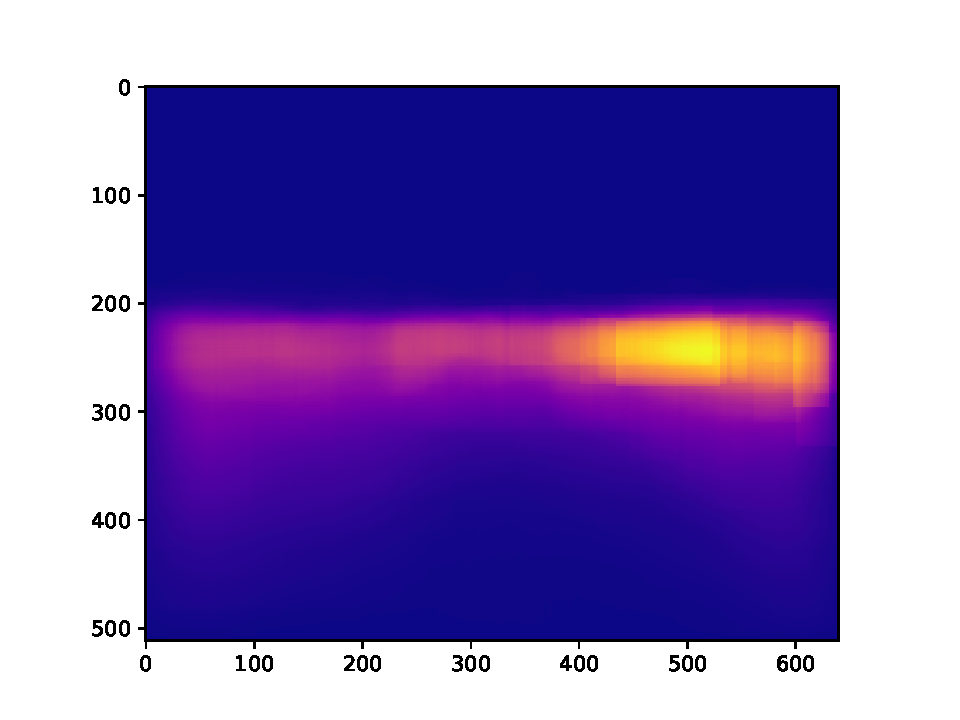
\includegraphics[width=0.8\textwidth]{images/graphic/heatmap.pdf}
    \caption{Heatmap riguardante la posizione dei pedoni}
    \label{fig:heatmap}
\end{figure}
\subsection{FLIR Thermal Starter Dataset}
\label{subsec:flirdataset}
Come già accennato in precedenza la documentazione riguardante questo dataset è molto stringata, limitandosi dunque ad una sola \href{https://www.flir.com/oem/adas/adas-dataset-form/}{pagina web} molto riassuntiva. Cercheremo in questa sezione di parlare degli aspetti che caratterizzano questo dataset.

Il dataset in questione offre immagini termiche con annotazioni e l'equivalente a colori non annotato. A differenza di \ref{subsec:kmpd} le due immagini non sono allineate, quindi non è possibile portare le annotazioni delle immagini termiche sulle immagini a colori.
Le immagini sono state acquisite tramite telecamere montate su una vettura e contiene un totale di 14453 immagini, di cui 10228 campionate da video di breve durata e 4224 provenienti da video di 144 secondi.
Tutte le immagini sono state acquisite su strade ed autostrade a Santa Barbara, in California. L'arco temporale varia da Novembre a Maggio, nello stessa quantità di giorno e notte. Il meteo è generalmente buono.

Le immagini termiche sono state scattate con una \textit{FLIR Tau2}, mentre quelle RGB con una \textit{FLIR BlackFly}. Entrambi i device sono stati impostati in maniera tale da avere lo stesso \ac{FOV} e per quanto riguarda il resto sono state lasciate entrambe alle impostazioni di default. 
Le videocamere sono state posizionate sullo stesso supporto a distanza di circa $1.9$ pollici (circa $4.8$ centimetri) l'una dall'altra. Il \textit{framerate} è di $2$ frame al secondo in scenari densi di annotazioni, mentre in scenari più tranquilli è stato deciso di scendere ad un frame al secondo.

Le annotazioni dove possibile ricalcano i codici adottati dal dataset \href{http://cocodataset.org/}{COCO}, ed hanno i seguenti codici:
\begin{itemize}
    \item 1 People: esseri umani.
    \item 2 Bicycles: biciclette e moticicli. Questa è l'unica categoria non consistente con il formato adottato da COCO.
    \item 3 Cars: automobili e veicoli piccoli.
    \item 18 Dogs: cani 
    \item 91 Other Vehicle: camion, rimorchi e imbarcazioni.
\end{itemize}

Le annotazioni sono state fatte manualmente da esseri umani ai quali è stato comunicato di fare \ac{BB} il più piccole possibili e che omettessero piccole parti di oggetti, accessori personali e parti occluse. Inoltre è stato comunicato di non annotare oggetti di piccole dimensioni o molto occlusi e persone delle quali si vede solo braccia o gambe.

\section{Addestramento iniziale di RetinaNet}
\label{sec:addestramento_iniziale_di_retinanet}
In questa sezione presenteremo i risultati iniziali dell'addestramento di RetinaNet sui due dataset descritti in sezione \ref{sec:dataset}. Per lo scopo è stata usata una versione di \textit{RetinaNet} implementata tramite \textit{Keras} reperibile in forma originale al seguente \href{https://github.com/fizyr/keras-retinanet}{link}. Durante lo sviluppo del lavoro di tesi le modifiche al codice originale sono state molteplici, tanto da aver richiesto un \textit{fork} della \textit{repository} originale reperibile al seguente \href{https://github.com/iskorini/keras-retinanet}{link}. Per tenere traccia dell'addestramento è stato usato \href{https://www.wandb.com}{\textit{Weight \& Biases}}.
\subsection{Transfer Learning}
\label{subsec:transfer_learning}
Inizialmente è stata usata la tecnica del \textit{Transfer Learning}. Una rapida spiegazione del significato di questa espressione ce la fornisce il libro \textit{Deep Learning} di \textit{Goodfellow et al} \cite{Goodfellow-et-al-2016}
\begin{quote}
    Transfer learning and domain adaptation refer to the situation where what has been learned in one setting is exploited to improve generalization in another setting.
\end{quote}
Per un'introduzione più dettagliata su cos'è il \textit{transfer learning} e sui vari tipi è stato preso spunto da \textit{A survey on Transfer Learning} di \textit{S. J. Pan} e \textit{Q. Yang} \cite{5288526}. 

La necessità di attuare tecniche di \textit{transfer learning} deriva dal fatto che molti modelli di Machine Learning lavorano bene solo sotto determinate assunzioni, soprattutto quella che i dati di addestramento e di test derivino dallo stesso spazio delle \textit{feature} e dalla stessa distribuzione. I problemi sorgono quando cambia la distribuzione, in quanto è necessario procedere ad una nuova fase di training. 

Le casistiche in cui il \textit{transfer learning} è applicabile sono molteplici, ad esempio l'analisi dei sentimenti, dove il compito è classificare le recensioni di un determinato prodotto in positive o negative. Per un compito del genere il primo passo da effettuare è la raccolta e l'annotazione di recensioni. Successivamente è necessaria una fase di addestramento di un modello usando come dati le recensioni precedentemente raccolte ed annotate.
Lo scopo è poter usare lo stesso modello per vari prodotti, in questo caso però si va incontro al problema che le distribuzioni dei dati su diversi prodotti possono differire anche di molto. La soluzione sarebbe quindi di annotare altre recensioni, ma richiederebbe uno sforzo notevole. L'idea è quindi di adattare un modello di classificazione, addestrato su alcuni prodotti, per aiutare la fase di addestramento su articoli differenti.
Le differenze tra processi di apprendimento tradizionali e \textit{transfer learning} sono mostrate in Figura \ref{fig:differences}.
\begin{figure}.
    \centering
    \subfloat[\label{fig:differencesa}]{
    \begin{tikzpicture}
        \node[circle, draw, ultra thick, fill=gray!20, minimum size=1.6cm](task1) {Task 1};
        \node[circle, draw, ultra thick, fill=gray!20, right = 0.7cm of task1, minimum size=1.6cm](task2) {Task 2};
        \node[circle, draw, ultra thick, fill=gray!20, right = 0.7cm of task2, minimum size=1.6cm](task3) {Task 3};
        \node[rectangle, draw, ultra thick, fill=gray!20, below = 1.5cm of task1](m1) {Modello};
        \node[rectangle, draw, ultra thick, fill=gray!20, below = 1.5cm of task2](m2) {Modello};
        \node[rectangle, draw, ultra thick, fill=gray!20, below = 1.5cm of task3](m3) {Modello};
        \draw[vecArrow] (task1) to (m1);
        \draw[vecArrow] (task2) to (m2);
        \draw[vecArrow] (task3) to (m3);
    \end{tikzpicture}
    \label{fig:differencesa}
    }
    \subfloat[\label{fig:differencesb}]{
    \begin{tikzpicture}[]
        \node[circle, draw, ultra thick, fill=gray!20, minimum size=1.6cm](task1) {Task 1};
        \node[circle, draw, ultra thick, fill=gray!20, right = 0.7cm of task1, minimum size=1.6cm](task2) {Task 2};
        \node[circle, draw, ultra thick, fill=gray!20, right = 0.7cm of task2, minimum size=1.6cm](task3) {Task 3};
        \path (task1) -- (task2) node[rectangle, draw, ultra thick, fill=gray!20, pos=.5,below=2.4cm] (m1) {Conoscenza};
        \node[rectangle, draw, ultra thick, fill=gray!20, below of = task3, right of = m1](m3) {Modello};
        \draw[vecArrow] (task1) to (m1);
        \draw[vecArrow] (task2) to (m1);
        \draw[vecArrow] (task3) to (m3);
        \draw[vecArrow] (m1) to (m3);
        \end{tikzpicture}
    }
    
    \caption{Differenze tra apprendimento tradizionale e transfer learning}
    \label{fig:differences}
\end{figure}

\paragraph{Notazione preliminare}
Per introdurre un po' più nello specifico le varie tipologie di \textit{transfer learning} è necessario definire alcuni concetti. Il primo di questi è il \textit{Dominio} $\mathcal{D}$, definito come una tupla $\mathcal{D} = \{\mathcal{X}, P(X)\}$, dove $\mathcal{X}$ è lo spazio delle \textit{feature} e $P(X) \text{ con } X = \{x_1, x_2, \dots, x_n\} \in \mathcal{X}$ è una distribuzione di probabilità marginale. In generale due domini possono essere considerati differenti se hanno differenti spazi delle \textit{feature} o distribuzioni differenti. 

Dato uno specifico dominio $\mathcal{D} = \{\mathcal{X}, P(X)\}$ è possibile definire il \textit{task}. Un \textit{task} $\mathcal{T}$ è una tupla $\mathcal{T} = \{\mathcal{Y},f(\cdot)\}$ con $\mathcal{Y}$ spazio dei \textit{label} e $f(\cdot)$ funzione di predizione. La particolarità del \textit{task} è il fatto che non è osservabile ma può essere appreso dai dati di addestramento, che consistono di una coppia $\{x_i, y_i\}$ con $x_i \in X$ e $y_i \in \mathcal{Y}$. Una volta completata la fase di addestramento dovrebbe essere possibile usare la funzione $f(\cdot)$ per predirre il label $f(x)$ corrispondente ad una nuova istanza $x$.

Chiameremo il dominio sorgente $\mathcal{D}_S$ ed il dominio target $\mathcal{D}_t$. In particolare avremo a disposizione anche i dati $D_S$ del dominio sorgente, definiti 
come $D_S = \{(x_{S_1}, y_{S_1}), \dots, (x_{S_n}, y_{S_n})\}$ tali che $x_{S_i} \in \mathcal{X}_S$ è l'istanza del dato e $y_{S_i} \in \mathcal{Y}_S$ è il corrispondente label. In maniera similare definiamo anche i dati del dominio target $D_T = \{(x_{T_1}, y_{T_1}), \dots, (x_{T_n}, y_{T_n})\} $ tali che $x_{T_i} \in \mathcal{X}_T$ è l'istanza del dato e $y_{T_i} \in \mathcal{Y}_T$ è il corrispondente label. 

Dire che due domini $\mathcal{D}_S$ e $\mathcal{D}_T$ implica che  o $\mathcal{X}_S \neq \mathcal{X}_T$ oppure $P_X(X) \neq P_T(X)$. In maniera del tutto analoga è possibile definire la differenza tra due \textit{task} $\mathcal{T}_S \text{ e } \mathcal{T}_T$. Nel caso in cui i due domini ed i due task sono uguali ci si riconduce ad un tradizionale problema di apprendimento. Quando invece c'è una relazione, implicita o esplicita, tra gli spazi delle \textit{feature} dei due domini si dice che il dominio sorgente e target sono in relazione tra di loro.
\paragraph{Tipologie di Transfer Learning} Prima di introdurre le varie tipologie di \textit{transfer learning} è necessario definire formalmente questo concetto e fare alcune premesse.
\begin{definition}{(Transfer Learning)}
    Dato un dominio sorgente $\mathcal{D}_S$, un task di apprendimento $\mathcal{T}_S$, un dominio target $\mathcal{D}_T$ ed un task di apprendimento $\mathcal{T}_T$, il transfer learning tenta di migliorare l'apprendimento di $f(\cdot)_T \in \mathcal{D}_T$ usando la conoscenza in $\mathcal{D}_S$ e $\mathcal{T}_S$, con $\mathcal{D}_S \neq \mathcal{D}_T$ o $\mathcal{T}_S \neq \mathcal{T}_T$.
\end{definition}
Quando si parla di \textit{transfer learning} bisogna mettere in conto tre problemi: \emph{cosa}, \emph{come} e \emph{quando} trasferire.
\begin{itemize}
    \item Cosa trasferire: quale parte della conoscenza bisogna trasferire tra domini o task sorgenti e target. In particolare possiamo dire che alcune conoscenze sono comuni tra i diversi domini, mentre altre sono specifiche. 
    \item Come trasferire: a questo problema pone una soluzione l'algoritmo di trasferimento della conoscenza.
    \item Quando trasferire: ci chiediamo in quali situazioni è realmente necessario applicare tecniche di \textit{transfer learning} ed in quali non è assolutamente necessario. Ad esempio in casi in cui i due domini sorgente e target non sono in relazione tra di loro il \textit{transfer learning} potrebbe non portare ad alcun risultato positivo. Si tende quindi sempre a parlare di \textit{transfer learning} dando per scontato che i due domini siano in qualche modo relazionati tra di loro, in quanto altrimenti non avrebbe senso andare oltre l'apprendimento tradizionale. 
\end{itemize}

Possiamo ora descrivere le tre categorie di \textit{transfer learning}:
\begin{itemize}
    \item \emph{Transfer Learning Induttivo}: il task target è differente dal task sorgente e non importa se il dominio sorgente ed il dominio target sono uguali o meno. Per indurre un modello predittivo oggettivo, da usare nel dominio target, sono necessari alcuni dati etichettati nel dominio sorgente. A seconda della tipologia ed alla quantità di annotazioni possiamo dividere questo tipo di \textit{transfer learning} in ulteriori due sottocategorie.
    \begin{itemize}
        \item Molti dati annotati nel dominio sorgente: ci si riconduce al caso del \textit{multitask learning}, tuttavia mentre lo scopo di quest'ultimo è operare bene in entrambi i domini, lo scopo del \textit{transfer learning} induttivo è operare bene solamente sul dominio obbiettivo.
        \item Nessun dato annotato nel dominio sorgente: le similarità in questo caso ci portano a pensare al \textit{self-taught learning}, dove le annotazioni tra il dominio sorgente ed obbiettivo sono totalmente differenti, e quindi non direttamente utilizzabili. 
    \end{itemize}
    \item \emph{Transfer Learning Trasduttivo (si traduce così "transductive"?)}: in questo caso il task obbiettivo ed il task sorgente sono i medesimi, mentre i domini sono differenti. Abbiamo quindi molti dati annotati nel dominio sorgente e nessuna annotazione nel dominio obbiettivo. Possiamo a sua volta dividere questa categoria in ulteriori due sottocategorie.
    \begin{itemize}
        \item Gli spazi delle feature tra sorgente e obbiettivo sono diffrenti, più formalmente abbiamo $\mathcal{X}_S \neq \mathcal{X}_T$
        \item Gli spazi delle feature tra sorgente e obbiettivo sono gli stessi, ma cambia la distribuzione di probabilità marginale, quindi $P(X_S) \neq P(X_T)$. Quest'ultimo caso è chiamato anche \emph{Domain Adaptation}.
    \end{itemize}
    \item \emph{Transfer Learning non supervisionato}: il task obbiettivo è differente dal task sorgente, ma hanno una qualche tipo di relazione tra di loro. Tuttavia l'attenzione si focalizza sul risolvere compiti di apprendimento non supervisionati nel dominio obbiettivo, come possono essere il \textit{clustering}, \textit{dimensionality reduction} o \textit{density estimation}. Non abbiamo quindi annotazioni né nel dominio sorgente, né nel dominio obbiettivo.
\end{itemize}
In Tabella \ref{table:TransferLearning} sono riassunte tutte le caratteristiche principali delle varie categorie di \textit{transfer learning}.
%TODO: SISTEMARE TABELLA
\textbf{SISTEMARE TABELLA \ref{table:TransferLearning}}
\begin{table}[]
    \centering
    \makebox[\textwidth]{
    \begin{tabular}{|c|c|c|c|c|}
    \hline
    Tipologia          & Similarità           & Annotazioni Sorgente & Annotazioni Target & Campo di applicabilità               \\ \hline
    Induttivo          & Multitask Learning   & SI                           & SI                         & Regressione e Classificazione        \\ \cline{2-5} 
                       & Self-taught Learning & NO                           & SI                         & Regressione e Classificazione        \\ \hline
    Trasduttivo        & Domain adaptation    & SI                           & NO                         & Regressione e Classificazione        \\ \hline
    Non supervisionato & 46501                & NO                           & NO                         & Clustering, dimensionality reduction \\ \hline
    \end{tabular}}
    \caption{Schema riassuntivo delle categorie di Transfer Learning}
    \label{table:TransferLearning}
\end{table}
\subsection{Addestramento sulle immagini RGB}
Per il primo esperimento è stato deciso di effettuare un training di \textit{RetinaNet} partendo dai pesi della rete precedentemente addestrata sul dataset di \href{http://cocodataset.org/}{COCO}. Il dataset utilizzato è \ac{kmpd}, descritto precedentemente in \ref{subsec:kmpd}. Il motivo è legato al fatto che è l'unico dataset a nostra disposizione a disporre di annotazioni sulle immagini RGB.

Questa prima fase di addestramento è durata circa $40$ ore, e come si può vedere dal grafico in Figura \ref{fig:fine_tuning_1} è proceduta senza particolari problemi fino ad arrivare a convergenza intorno all'epoca 45. Le classi usate per l'addestramento sono solamente \textit{person} e \textit{cyclist}. È stato deciso di non prendere in considerazioni le rimanenti classi in quanto sono persone non ben distinguibili. Tutti gli esperimenti sono stati eseguiti su una macchina remota dotata di una \ac{gpu} \href{https://www.geforce.com/hardware/desktop-gpus/geforce-gtx-titan-x}{Nvidia Titan X}.

\begin{figure}[h]
    \centering
    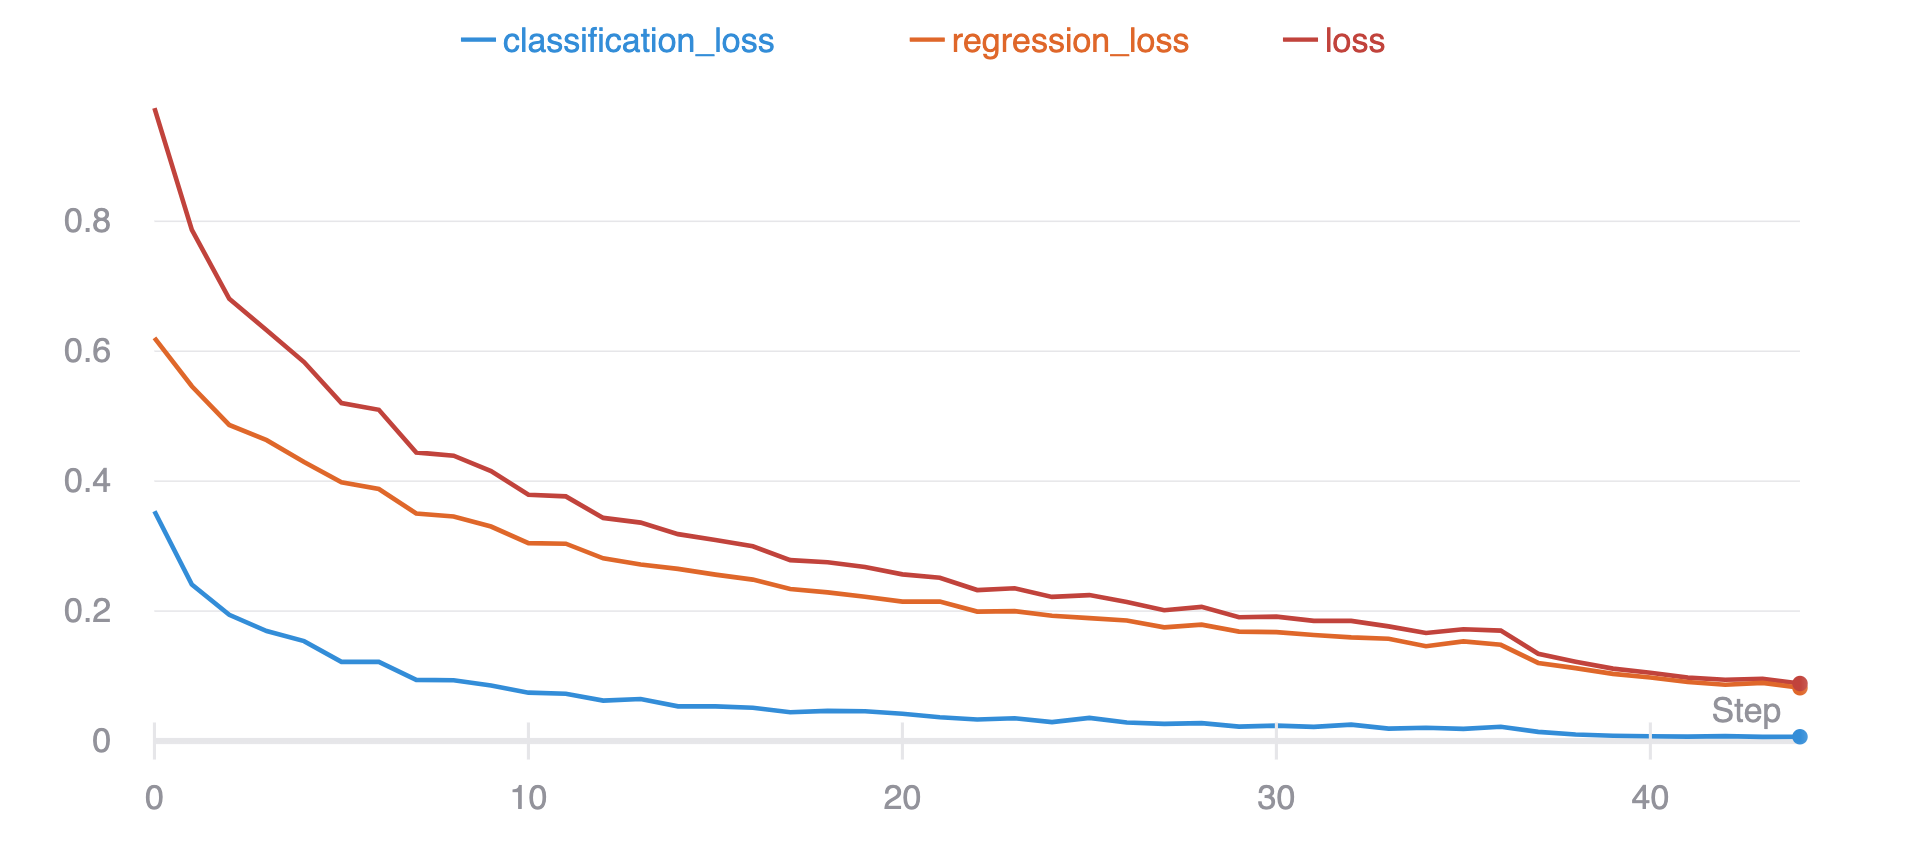
\includegraphics[width=\textwidth]{images/graphic/ruby-yogurt.png}
    \caption{Transfer learning da COCO a KAIST}
    \label{fig:fine_tuning_1}
\end{figure}

Dopo la fase di addestramento sono stati eseguite le valutazioni sulla parte di dataset adibita ai test. Inizialmente le classi utilizzate per i test sono le stesse usate per l'addestramento. I risultati complessivi vengono riassunti in Tabella \ref{table:first_test}. La \ac{map} mostrata nell'ultima riga della tabella è stata calcolata come media pesata secondo il numero di esempi all'interno del \textit{test set}.

\begin{table}[]
    \centering
    \begin{tabular}{|c|c|c|}
    \hline
                & $\#$ Istanze & mAP    \\ \hline
    Person      & 45195             & 0.4184 \\ \hline
    Cyclist     & 1396              & 0.1154 \\ \hline
    Complessivo & 46501             & 0.4093 \\ \hline
    \end{tabular}
    \caption{Test complessivo delle performance dopo l'addestramento}
    \label{table:first_test}
\end{table}

La valutazione è stata anche effettuata in maniera separata sia sulla parte di \textit{test set} diurna che notturna. I risultati sono mostrati in Tabella \ref{table:separate_test_day} e Tabella \ref{table:separate_test_night}. Come lecito aspettarsi, avendo visibilità limitata in notturna si ottengono risultati mediamente peggiori. In Figura \ref{fig:prediction_test_first} è possibile vedere un esempio di predizioni fatte sul \textit{test set}.

\begin{table}[]
    \centering
    \subfloat[Giorno\label{table:separate_test_day}]{
        \begin{tabular}{|c|c|c|}
        \hline
                    & $\#$ Istanze & mAP    \\ \hline
        Person      & 33688             & 0.4493 \\ \hline
        Cyclist     & 818               & 0.2015 \\ \hline
        Complessivo & 34506             & 0.4434 \\ \hline
        \end{tabular}
    }
    \subfloat[Notte\label{table:separate_test_night}]{
        \begin{tabular}{|c|c|c|}
        \hline
                    & $\#$ Istanze & mAP    \\ \hline
        Person      & 11507             & 0.3281 \\ \hline
        Cyclist     & 578               & 0.0029 \\ \hline
        Complessivo & 12085             & 0.3125 \\ \hline
        \end{tabular}
    }
    \caption{Risultati della valutazione separata}
    \label{table:separate_test}
\end{table}

\begin{figure}[]
    \centering
    \makebox[\textwidth]{
    \subfloat{
        \begin{minipage}[b][][t]{.3\textwidth}
        \centering
        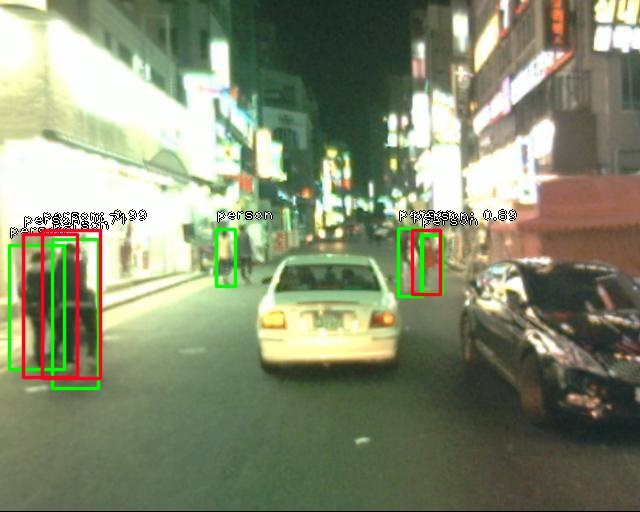
\includegraphics[width=.8\textwidth]{images/examples/first_test/I00011.jpg}
        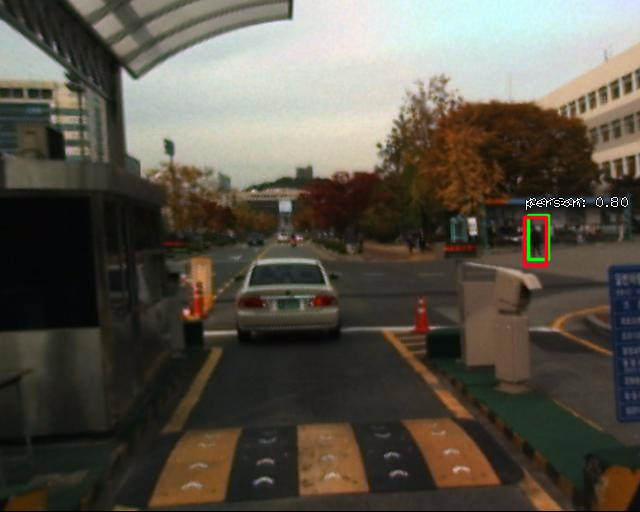
\includegraphics[width=.8\textwidth]{images/examples/first_test/I00146.jpg}
        \end{minipage}
    }%
    \subfloat{
        \begin{minipage}[b][][t]{.3\textwidth}
        \centering
        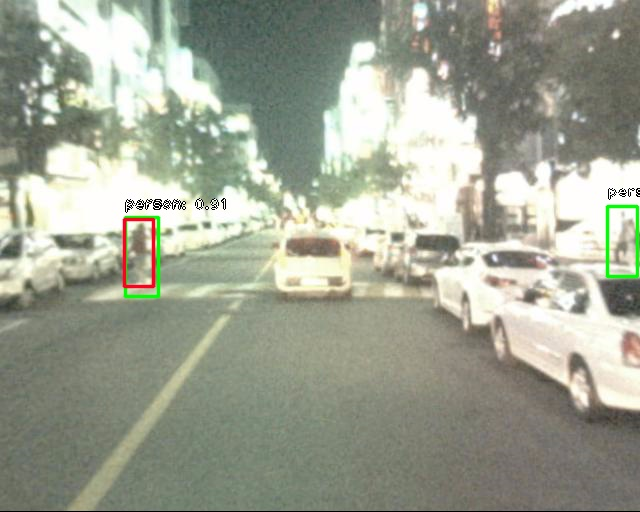
\includegraphics[width=.8\textwidth]{images/examples/first_test/I00222.jpg}
        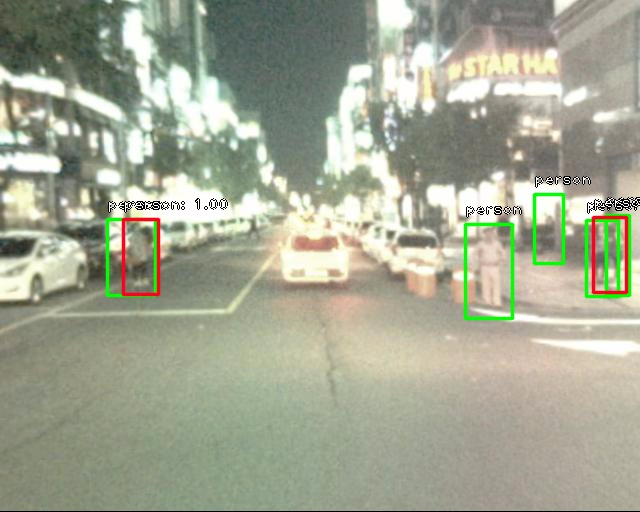
\includegraphics[width=.8\textwidth]{images/examples/first_test/I00159.jpg}
        \end{minipage}
    }
    \subfloat{
        \begin{minipage}[b][][t]{.3\textwidth}
        \centering
        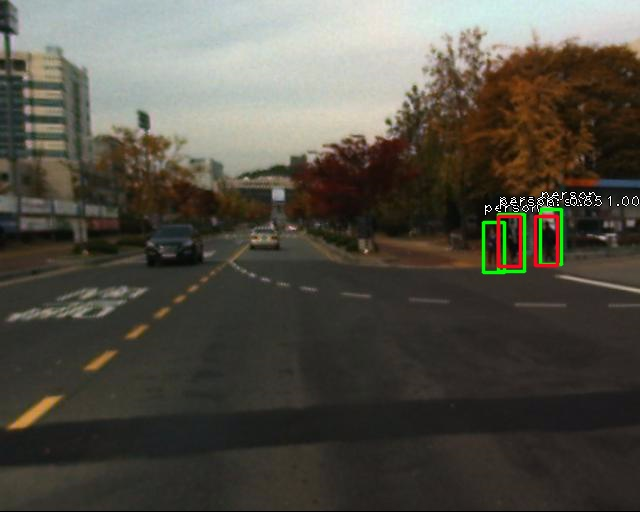
\includegraphics[width=.8\textwidth]{images/examples/first_test/I00265.jpg}
        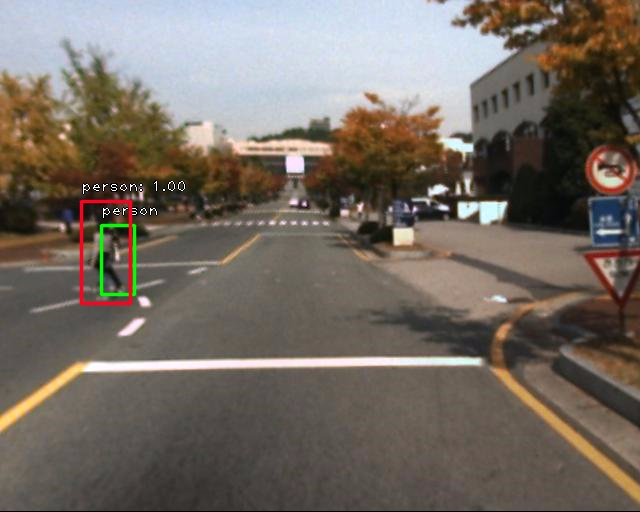
\includegraphics[width=.8\textwidth]{images/examples/first_test/I00599.jpg}
        \end{minipage}
    }
    \subfloat{
        \begin{minipage}[b][][t]{.3\textwidth}
        \centering
        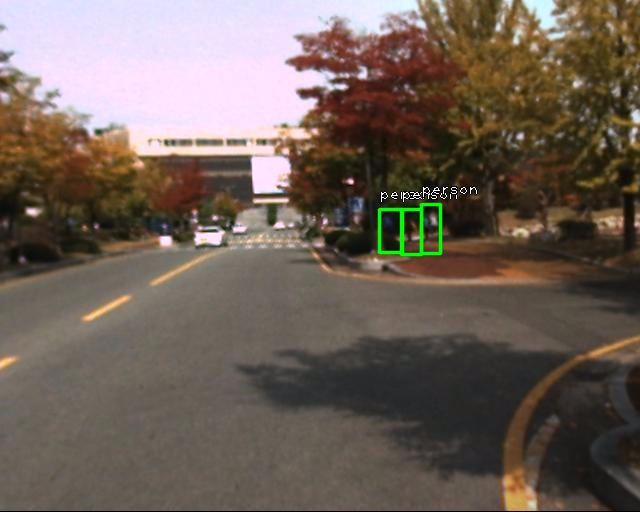
\includegraphics[width=.8\textwidth]{images/examples/first_test/I01314.jpg}
        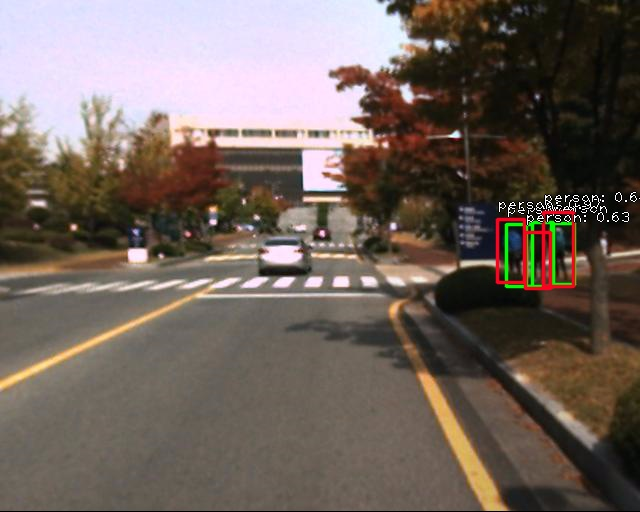
\includegraphics[width=.8\textwidth]{images/examples/first_test/I01512.jpg}
        \end{minipage}
    }
    }
    \caption{Esempio di predizioni, in verde la \textit{ground truth} in rosso le predizioni.} 
    \label{fig:prediction_test_first} 
\end{figure}


Il successivo step della valutazione è stato effettuato su più classi, per questa comparazione delle performance è stata presa in considerazione anche la classe \textit{people}, ma rinominandola in \textit{person} in maniera tale da farla digerire \textbf{rivedere questo periodo} alla rete già addestrata.
\textbf{INSERIRE VALUTAZIONE EFFETTUATA CON TUTTE LE CLASSI}

%-----------------GLOSSARIO ED ACRONIMI------------------------
\addcontentsline{toc}{chapter}{Acronimi}
\chapter*{Acronimi}
\begin{acronym}[CAGD]
    \acro{map}[mAP]{Mean Average Precision}
    \acro{kmpd}[KAIST MPD]{KAIST Multispectral Pedestrian Dataset}
    \acro{gpu}[GPU]{Graphics Processing Unit}
    \acro{KAIST}[KAIST]{Korea Advanced Institute of Science and Technology}
    \acro{FOV}[FOV]{Field of View}
    \acro{BB}[BB]{Bounding Box}
    \acro{RNN}[RNN]{Recurrent Neural Network}
    \acro{TPU}[TPU]{Tensor Processing Unit}
    \acro{CNN}[CNN]{Convolutional Neural Network}
    \acro{FCN}[FCN]{Fully Convolutional Network}
    \acro{RNN}[RNN]{Recurrent Neural Network}
    \acro{NMS}[NMS]{Non-Maximum Suppression}
    \acro{HNM}[HNM]{Hard Negative Mining}
    \acro{YOLO}[YOLO]{You Only Look Once}
    \acro{VOC}[VOC]{Pascal Visual Object Classes}
    \acro{ILSVRC}[ILSVRC]{ImageNet Large Scale Visual Recognition Challenge}
    \acro{MSCOCO}[MS-COCO]{Microsoft - Common Object in COntext}
    \acro{OID}[OID]{Open Images Detection}
\end{acronym}

%-----------------BIBLIOGRAFIA---------------------------------

\bibliography{bibliography}
\bibliographystyle{unsrt}



%--------------------------------------------------------------
\end{document}
%--------------------------------------------------------------